% !TeX root = /../Report.tex

\chapter{Experiments and Results}\label{sec:experiments}

\section{Experiment Setup}\label{sec:setup}
The hardware of the experiment setup consisted on a computer running the Matlab graphic simulation, the four master devices (Remote, Keyboard, Remote and CatheterLike) and an Arduino board, used to read the sensors of the devices (The keyboard was connected directly to the computer) and communicated with Matlab through USB serial. The diagram is shown in figure~\ref{img:expsetup}.\\

\begin{figure}[ht]
   \centering
   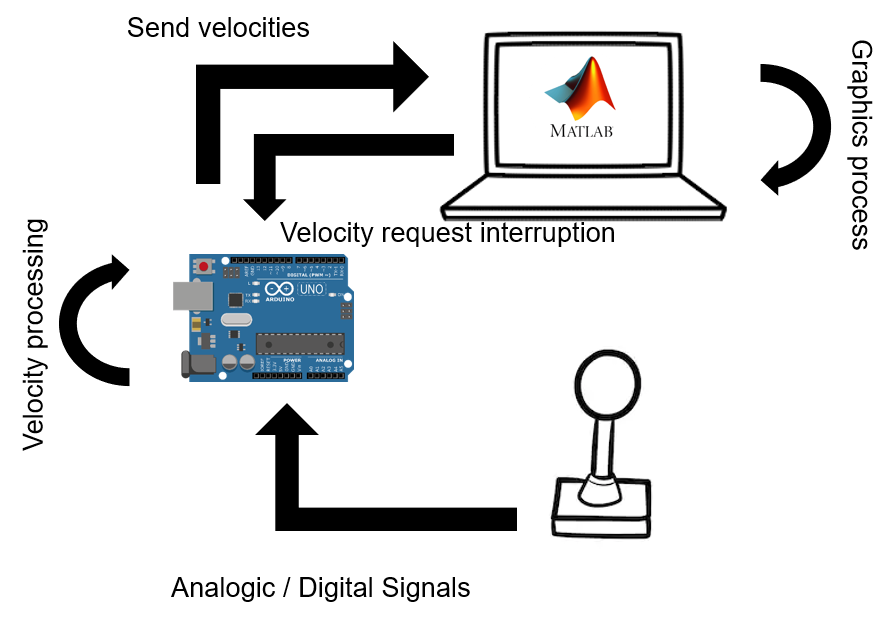
\includegraphics[width=0.7\textwidth]{img/expsetup.PNG}
   \caption{Experiment setup communication diagram}
   \label{img:expsetup}
\end{figure}

\section{Graphic Environment}\label{sec:environment}
The graphic environment is fully developed on Matlab, it consists on a representation of a catheter (With a green square following the tip) in a simulated fluoroscopy image, as surgeons would see it in the operation room, figure~\ref{img:graph}. This means the image showed on screen is a 2D black and withe plain representation. The catheter can be moved in its 2 DOF, being the 1st DOF the axial movement (defined in simulation by the Y coordinate), the catheter would move up and down only. The 2nd DOF is the rotation (defined in simulation as radians starting from the left most possible position of the catheter's tip), which is translated to a left and right movement on the screen.\\

Since the 2nd DOF is defined by the rotation (in radians) of the catheter, some dynamics are implicitly stated in the simulation during the left to right movements. Since the image shown is intended to be a 2D representation of an actual 3D catheter in real life, when the catheter is rotating over its own axis a sinusoidal movement can be observed, moving slower when the tip of the catheter is on the most left/right side of the screen. Thus, moving fast when the tip is near the center of the catheter.\\

\begin{figure}[ht]
   \centering
   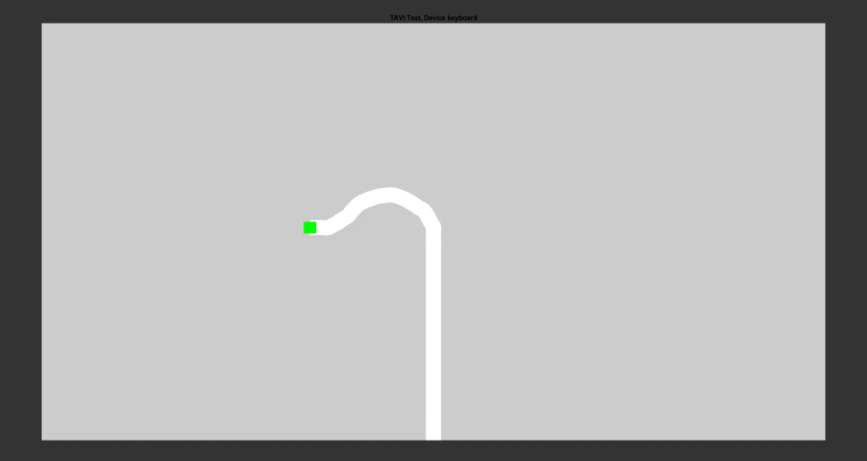
\includegraphics[width=0.7\textwidth]{img/graph.PNG}
   \caption{Default experiment graphic environment}
   \label{img:graph}
\end{figure}

\section{MATLAB/Arduino Interface}\label{sec:matardinter}
The Arduino board and Matlab are connected through USB serial communication. The Arduino board is responsible to sense the devices' sensors. When the Matlab simulation starts, Matlab sends the necessary commands to Arduino in order to set it up for the specific device that is going to be in use, after this the Arduino board start to capture the states of the sensors instantly.\\

Matlab simulation runs in a loop after setting up all the initial conditions. First it requests the Arduino board for the current states of the device. After it updates the graphics accordingly with the movements reported by Arduino. Lastly it stores the states in a log file, for later data analysis.\\

The Arduino board is programed with serial communication interruptions, which means it is constantly getting the current states of the device and storing them into a buffer. Once the Matlab code request for the information, the Arduino board code will be interrupted in order to send the last saved states from the device, once this is done the Arduino board will go back to its state reading task.\\

The only device that works in a different fashion is the keyboard, which is connected directly to the computer through USB. This device interrupts Matlab directly when one of the keys is pressed and stores the device state directly in the simulation environment. In order to avoid adding/subtracting external latency, even do the Keyboard does not interact directly with the Arduino board, the simulation in Matlab runs the communication with the Arduino board, which returns by default the constant from equation~\ref{eq:1steq}. The constant form equation~\ref{eq:1steq} is substituted by the keyboardConsat defined in equation ~\ref{eq:4theq}, being \{-1,0,1\} the possible states of keyboardMatlabState. Then the specific equation for the keyboard changes from~\ref{eq:1steq} to~\ref{eq:5theq}.\\

\begin{equation}
   \scalebox{1.2}{$outputVel=keyboardConst=constant*keyboardMatlabState$}
   \centering
   \label{eq:4theq}
\end{equation}

\begin{equation}
   \scalebox{1.2}{$outputVel=outputVel=keyboardConst+keyboardConst*pressedTime$}
   \centering
   \label{eq:5theq}
\end{equation}


\section{Arduino/Device Interface}\label{sec:arddevinter}
The Arduino board has analogical and digital input in which the devices are directly connected to, according each device sensor types. Once the Arduino board is initialized by Matlab, readings to the corresponding inputs are performed and processed according to the programed mapping type (see section~\ref{sec:mapping}). The processes information is stored in a buffer and the loop keeps running in the same way.\\

\section{Physical Setup}\label{sec:physical}
All the experiments were run in the same environment under the same conditions. An external monitor was setup to run the graphic simulation over a desk with a chair for the experiment candidate to sit. Every device was presented in front the candidate to be taken when necessary according the running experiment, as shown in figure~\ref{img:setupphy}.\\

All the simulations start only once the candidate had perform the first movement, in that moment the simulation starts recording data, and the simulation time or the goal is reached, it closes itself and immediately launches the next simulation, waiting for the candidate to perform the first movement again, until all the repetitions are finish.\\

\begin{figure}[ht]
   \centering
   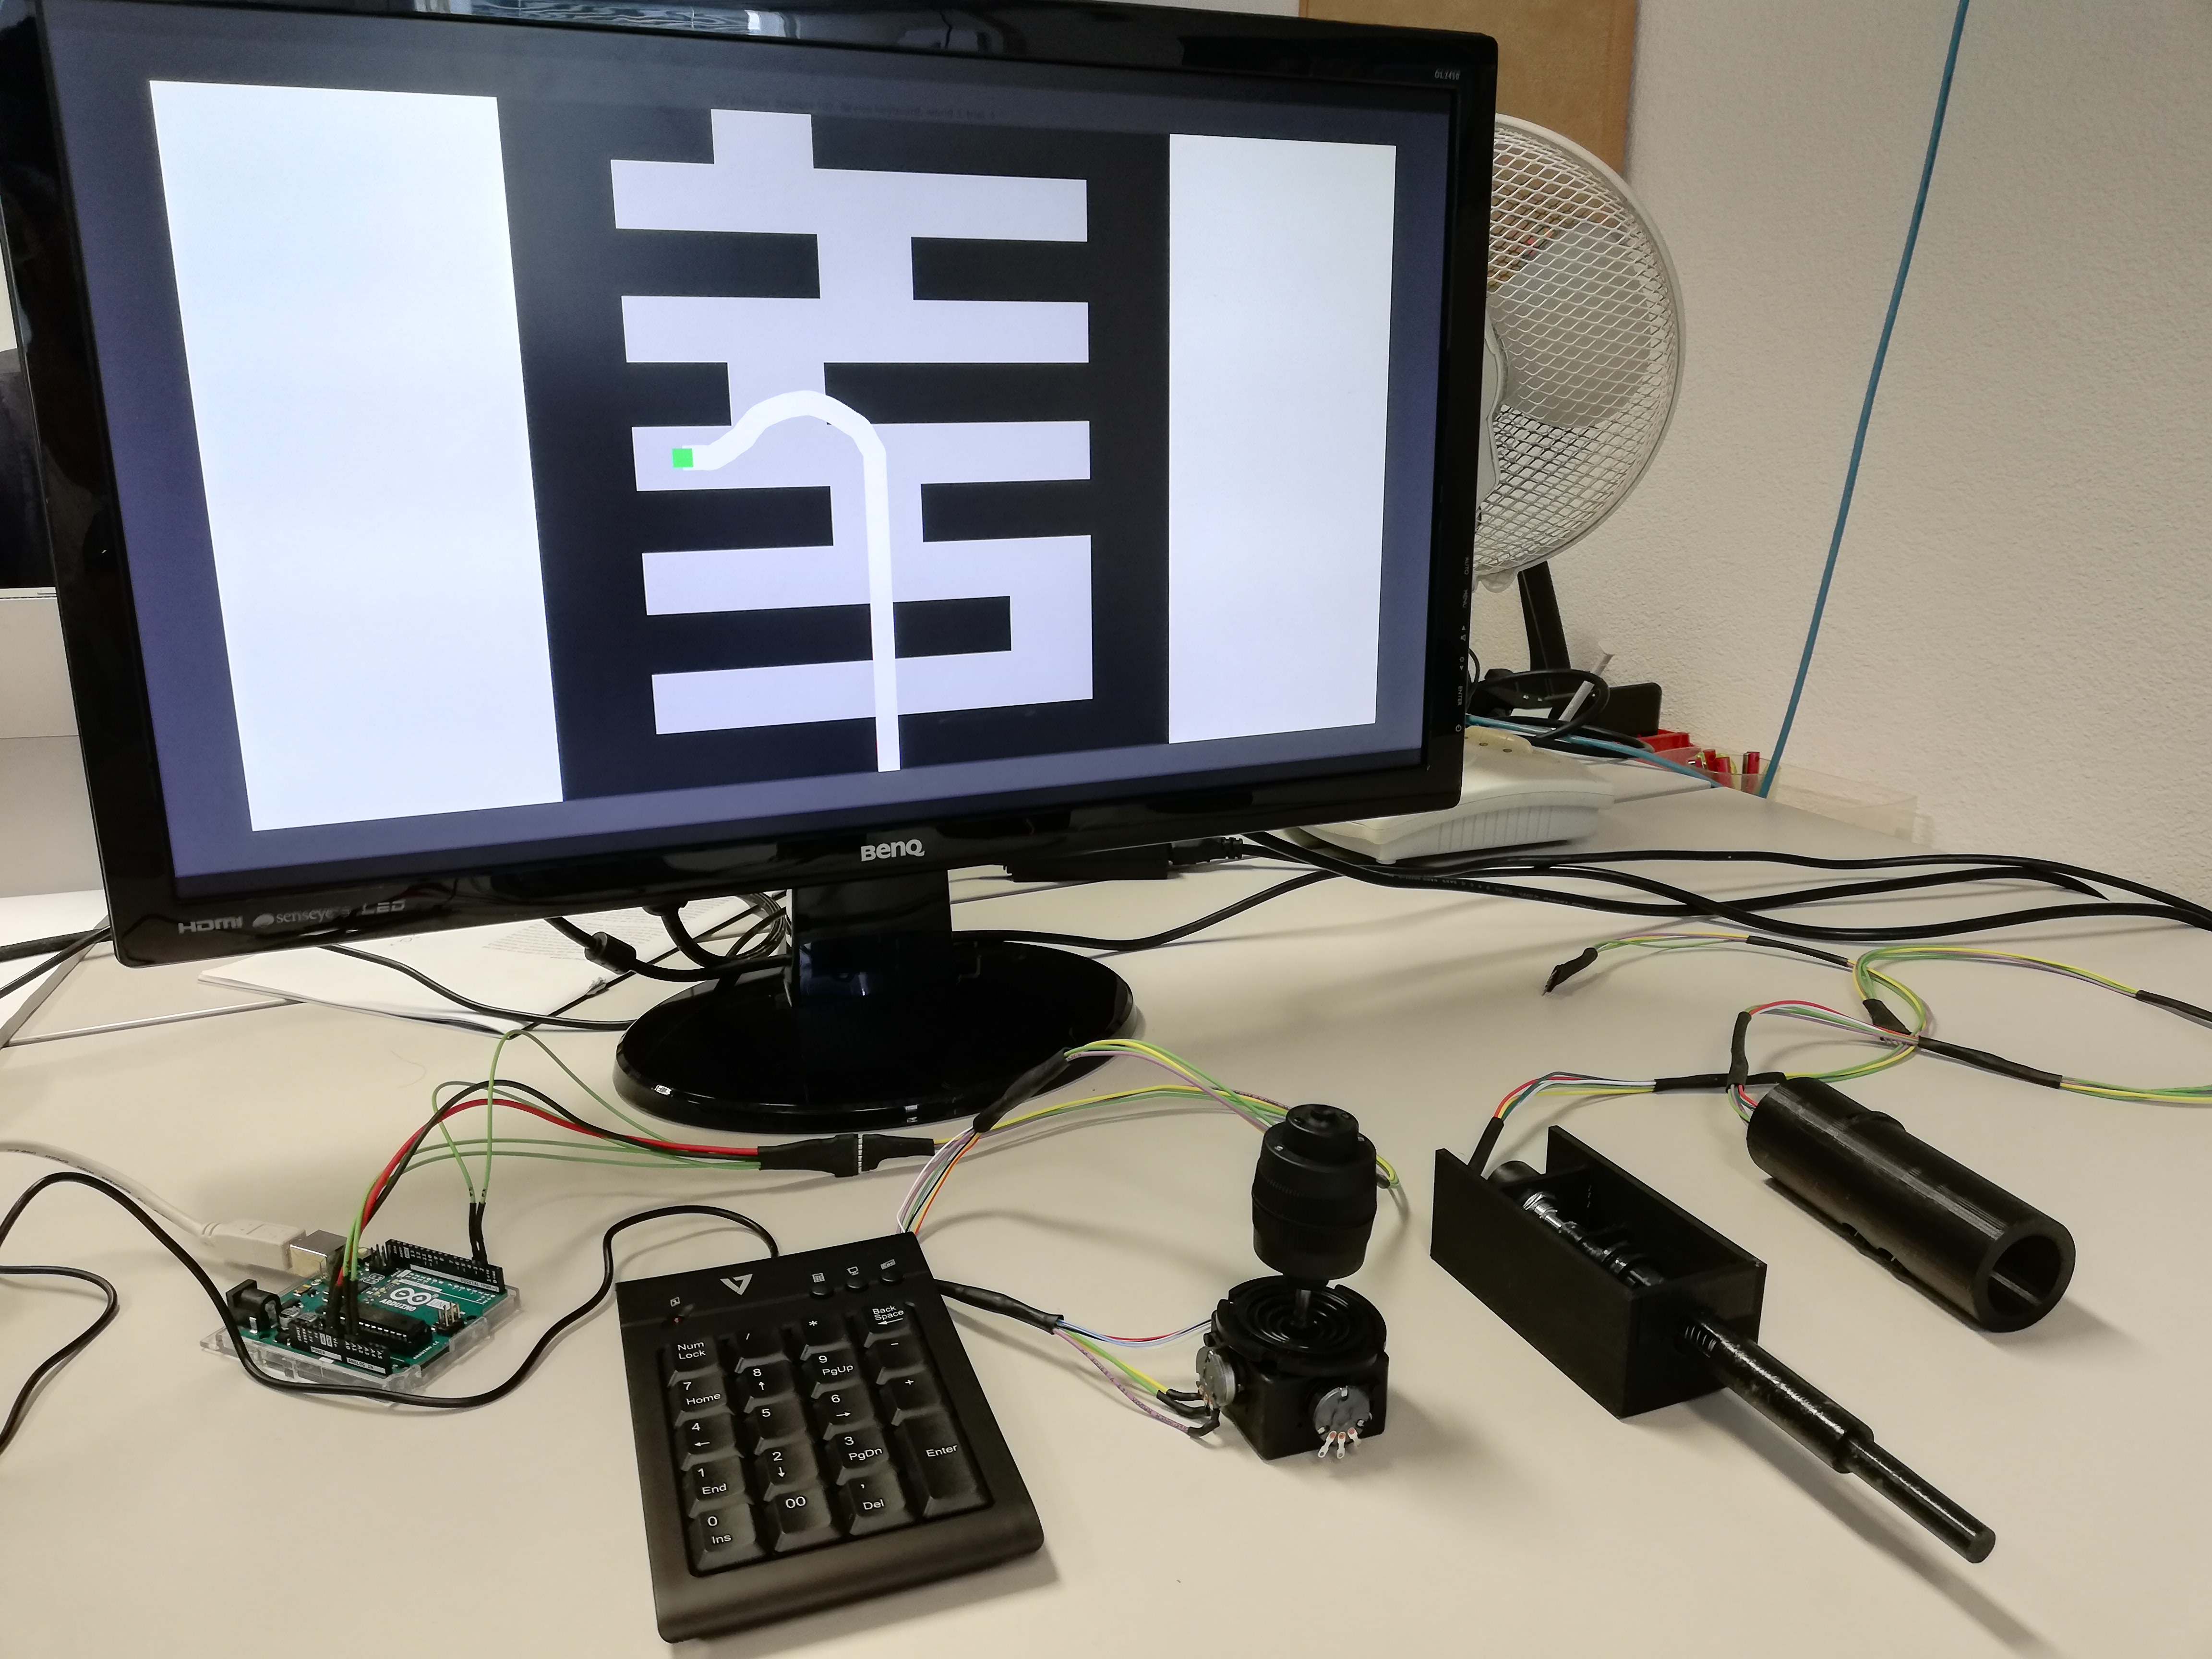
\includegraphics[width=0.7\textwidth]{img/setup.jpg}
   \caption{Physical setup environment used for the experiments}
   \label{img:setupphy}
\end{figure}

\section{Participants Statistics}\label{sec:partstats}
The experiment was conducted by 15 participants, from the 15 participants:
\begin{itemize}
\item  Only 1 of the participants was an expert surgeon in TAVI procedure
 \item The average age of the participants is: 30.23
 \item 46.15 were Male
 \item 	53.85 were Female
\end{itemize}


\section{Instructions}\label{sec:instructions}
Before initiating the experiments, a sheet with the instructions set as the one shown in appendix~\ref{sec:apinst} was handed to each one of the participants.\\


\section{Practice Round}\label{sec:pratround}
Before any experiment was performed, each participant had time to try and play with every device and how it interacts with the graphic simulation on each one of the DOF. An empty world simulation was displayed as shown in figure~\ref{img:graph}. The devices were randomly selected and handed to the participant, who could manipulate the simulated catheter until he would decide to stop or maximum 2 minutes had passed.\\


\section{Experiment 1st and 2nd DOF}\label{sec:1stexp}
\subsection{Overview}\label{subsec:1stover}
This experiment was designed to test the performance of the 1st DOF and 2nd DOF of every device independently. The objective is to try to collocate the tip of the catheter (green square) inside a target (red square) that is only moving up and down for the 1st DOF experiment (figure~\ref{img:1stexp}) and left to right for the 2nd DOF experiment (figure~\ref{img:2ndexp}). The target is always initially collocated above the initial tip of the catheter position for the 1st DOF and to the right of the initial tip of the catheter position for the 2nd DOF experiment. The target starts moving automatically once the simulation detects the first movement of the user, following a predefined path for 10 seconds.\\

For each DOF three different predefined paths (worlds) for the target were created, trying to cover two main purposes, the first one was to exploit the capabilities of every device, reaction time, resolution, change of direction, acceleration and deceleration. The second purpose was to simulate movements surgeons would face in a normal TAVI procedure. For the 1st DOF having to pull back rapidly after being moving front and small precise movements when placing the new valve (preventing PVA~\cite{pvl}~\cite{pvl2}) or trying to cross the aortic valve. On the other hand, for the 2nd DOF having to rotate to avoid a blockage in the artery or contacting with the wall of the aortic artery, and small precise rotation movements surgeons need to perform as technique for crossing the aortic valve~\cite{raptech}~\cite{anatomic}.\\

During the 10 seconds of simulation the RMSE between the tip of the catheter and the target is recorded in X and Y coordinates independently. This measurement was selected as it encloses information and gives insight of the experiment purpose previously mentioned.\\

For each one of the DOF every participant had to complete five times each one of the three target's predefined paths, which means 15 randomly order repetitions per device. The repetitions were executed all, one device at a time; however, the devices were ordered randomly at the beginning of the experiment. Also, the order on which every DOF experiment was performed, was randomized for every participant.\\

\begin{figure}[ht]
   \centering
   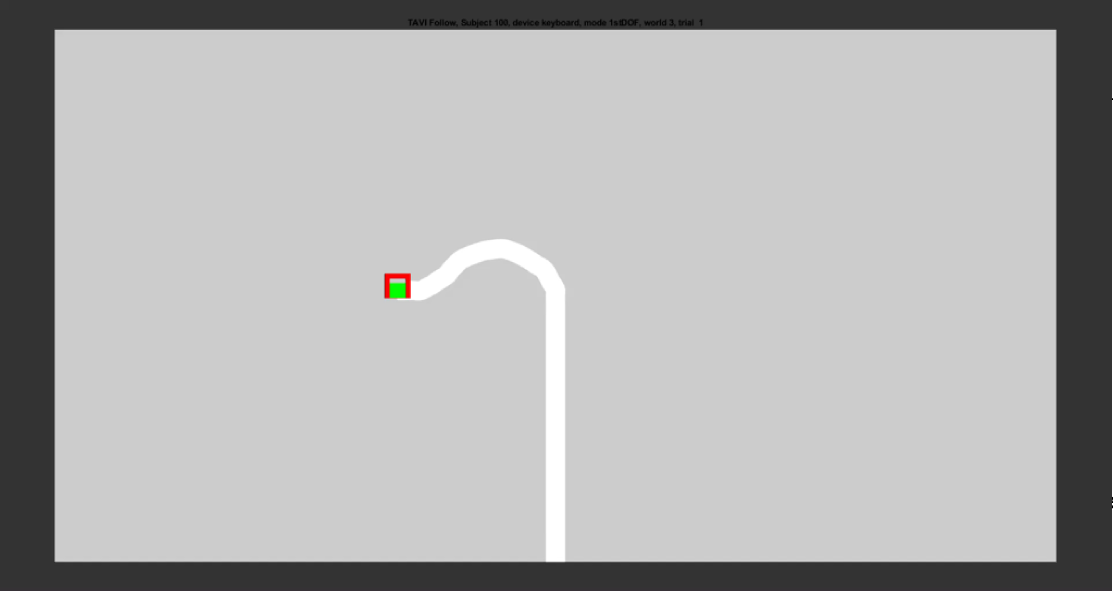
\includegraphics[width=0.8\textwidth]{img/1stexp.PNG}
   \caption{Initial state of the 1st DOF experiment}
   \label{img:1stexp}
\end{figure}

\begin{figure}[ht]
   \centering
   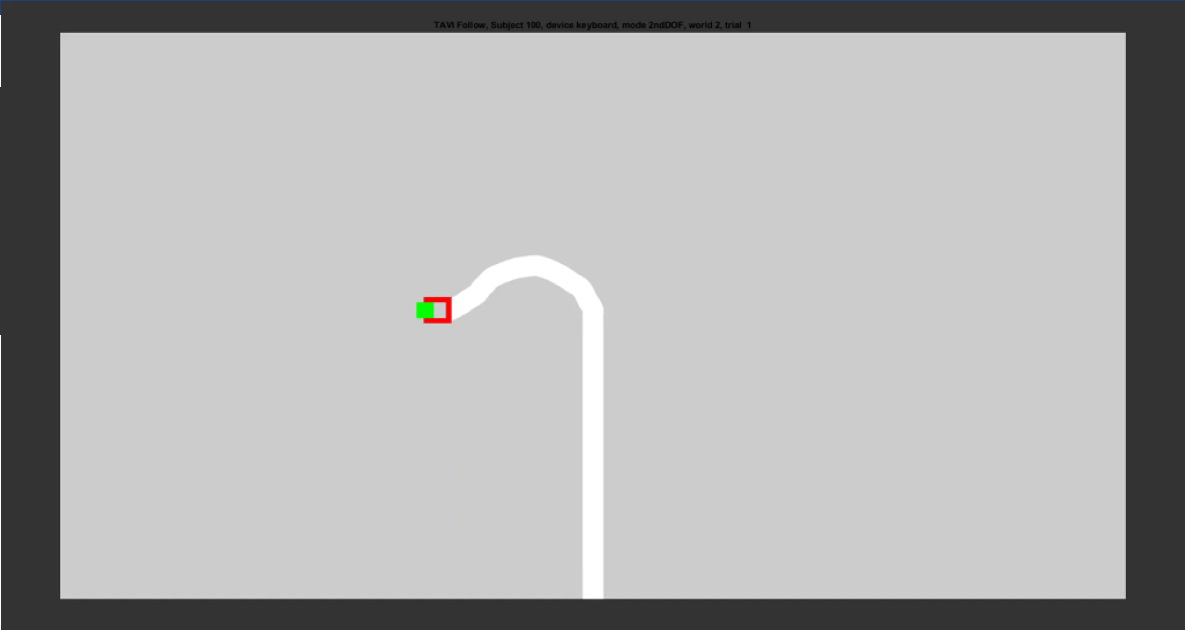
\includegraphics[width=0.8\textwidth]{img/2ndexp.PNG}
   \caption{Initial state of the 2nd DOF experiment}
   \label{img:2ndexp}
\end{figure}

\subsection{Results}\label{subsec:1stres}
All the data from the 15 participants was gathered and the RMSE in both coordinates X and Y for each one of the two DOF computed.\\

As can be observed in figure~\ref{img:1stAvgError}, the 1st DOF experiment shows that the Joystick device has a better performance than the rest of the devices at every different world, followed by the keyboard. However, in figure~\ref{img:1stError} when showing all the samples from the 3 words together, two important things are observed. First, the joystick device seems to still show a better performance, but this cannot be concluded when comparing with the keyboard, due to interaction P-Value of 0.006. On the second place, the Joystick device can be observed a high number of atypical values far away from the box plot, which at first seemed to be failed experiments. However, if those atypical values are traced, the majority of them belong to the first trials of different participants. Thus, if each number of trials is plotted separately as in figure~\ref{img:1stTrainNoExp} (a participant without previous training using Joysticks), a pronounced training curve can be observed. On the other hand, if we plot the same information from a participant that reported experience with the type of the devices used for the experiment as in figure~\ref{img:1stTrainExp}, can be observed the superior performance of the Joystick again followed by the keyboard at every attempt.\\

Another important thing to look at, is the accidental activation error, which means movements in the DOF that was not being tested at each experiment. In order to quantify this involuntary movements, since some of them were too small to be quantified, a percentage of trials where and activation error was present was calculated, as can be observed in figure~\ref{img:1stAct}. It is intuitive that the Keyboard has 0\% due to its digital characteristics, something that would be expected as well from the Remote device, however, that was not the case, since 2.7\% of the cases had an activation error, which can be attributed to experiment errors or issues with the ergonomics of the device. Finally, it can be observed that the catheter had the higher activation error, followed by the joystick.\\

On the 2nd DOF the figure~\ref{img:2ndAvgError} shows that the keyboard had a better performance at every world than any other device, without a clear differentiation between the other three. Also, in the boxplots of figure~\ref{img:2ndError} can be observed how the Joystick, Remote and Catheter devices have similar distributions, and the keyboard having a better performance with a P-Value of 4.5e-10.\\

The same training behavior as in the 1st DOF experiment can be observed in the 2nd DOF for some of the devices, as shown in figure~\ref{img:2ndTrainNoExp} from a candidate without experience manipulating devices. Also, in figure~\ref{img:2ndAct} the accidental activation error, of the 1st DOF in this case, shows a 0\% in the Keyboard and Remote (devices involving digital inputs in at least one of the two DOF), followed by the Joystick with 3.5\% of test cases and the Catheter with the worst performance with 8\%. Both devices with 0\% proven to be better than the Catheter with P-Value of 0.001, but failed to prove superiority with the Joystick due to an interaction P-Value of 0.03.\\

\begin{figure}[ht]
   \centering
   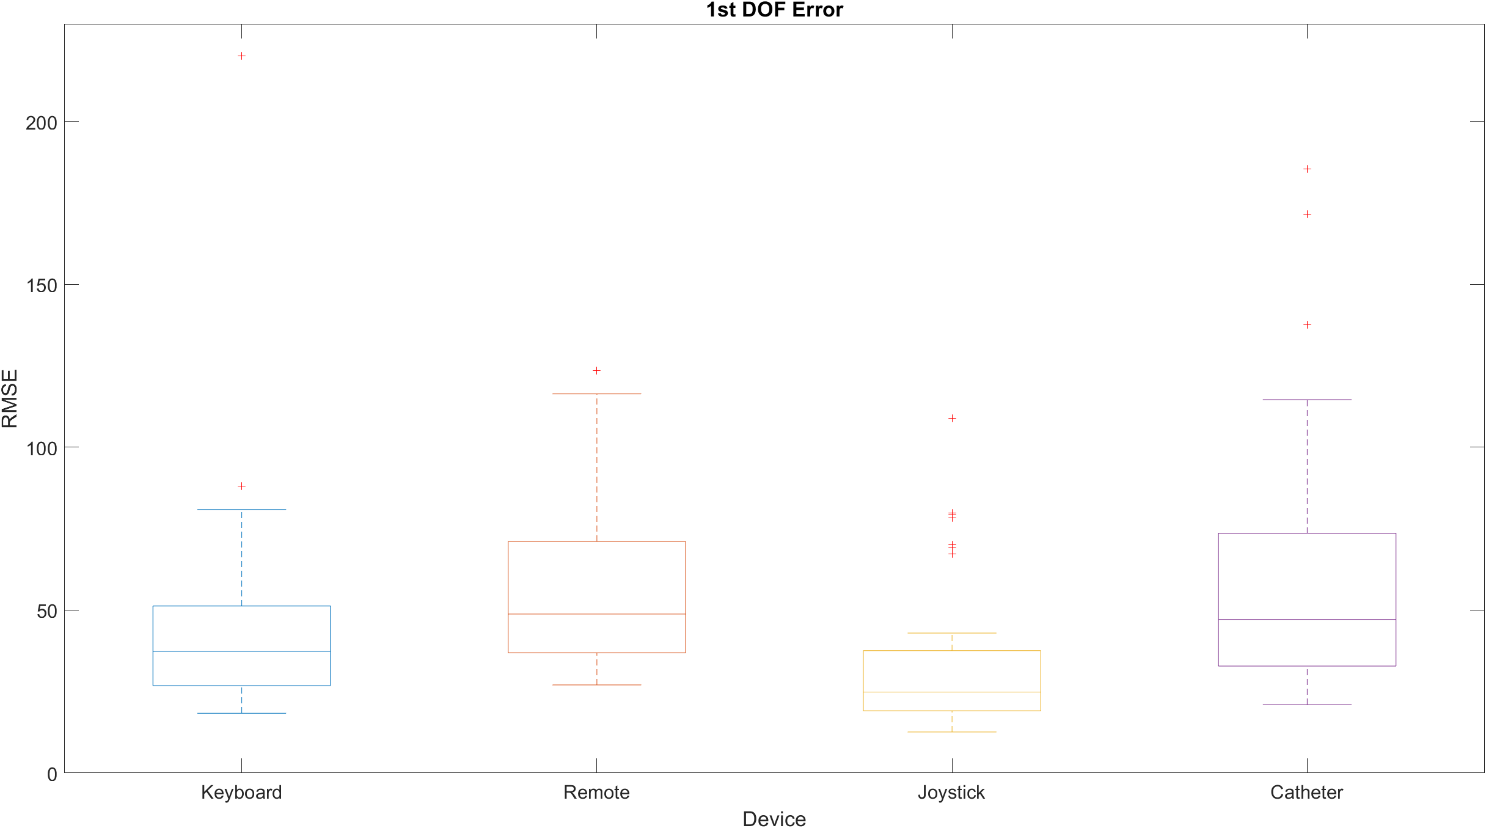
\includegraphics[width=1.0\textwidth]{img/1st/1stError.png}
   \caption{1st DOF RMSE per device across all worlds}
   \label{img:1stError}
\end{figure}

\begin{figure}[ht]
   \centering
   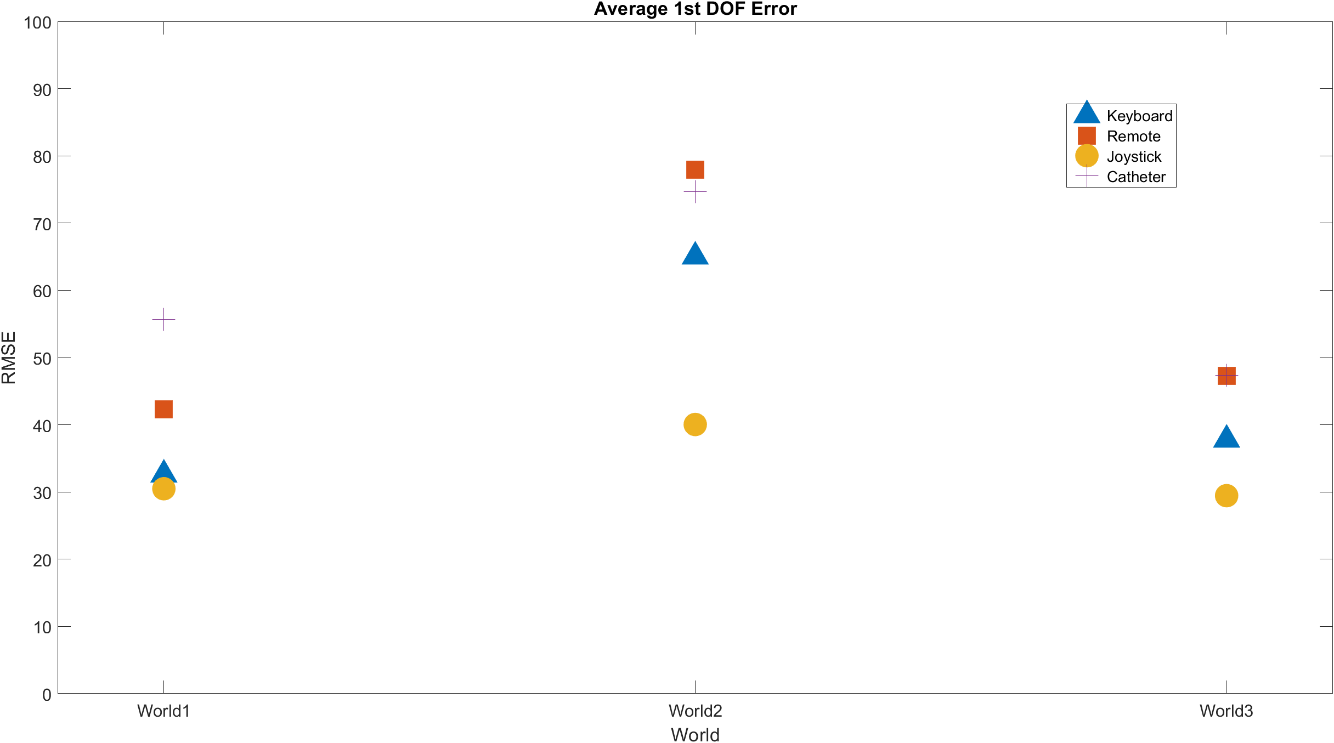
\includegraphics[width=1.0\textwidth]{img/1st/1stAvgError.png}
   \caption{1st DOF RMSE per device at each world}
   \label{img:1stAvgError}
\end{figure}

\begin{figure}[ht]
   \centering
   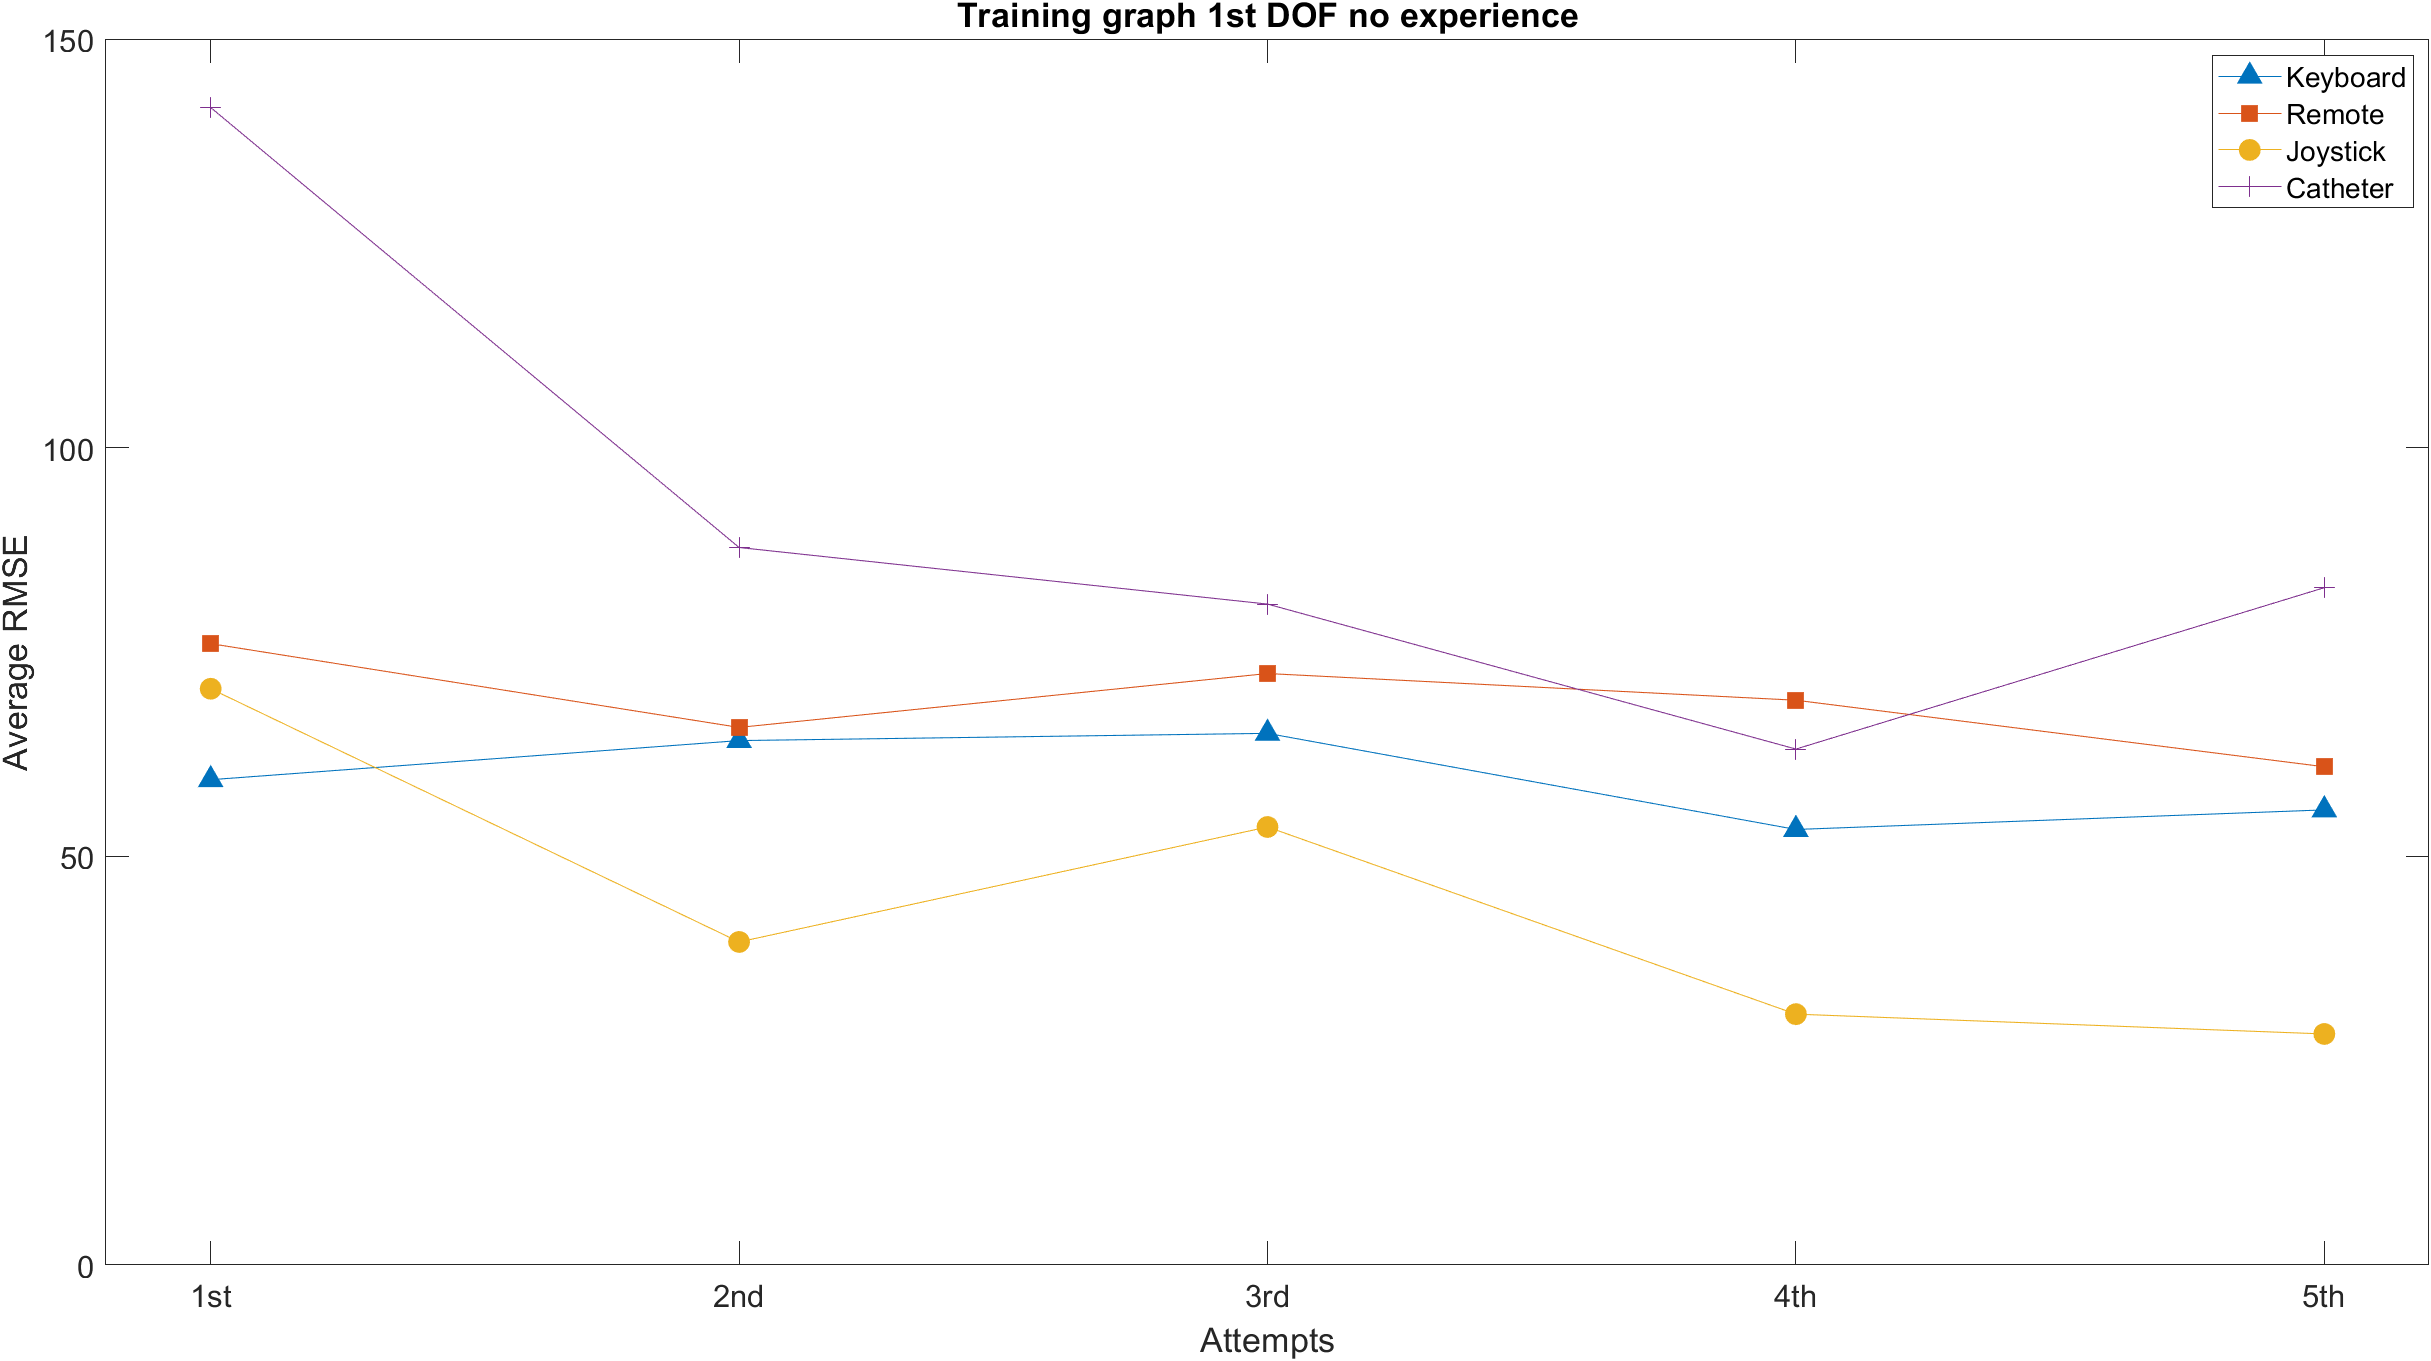
\includegraphics[width=1.0\textwidth]{img/1st/1stTrainNoExp.png}
   \caption{1st DOF RMSE per attempt, participant with no experience}
   \label{img:1stTrainNoExp}
\end{figure}

\begin{figure}[ht]
   \centering
   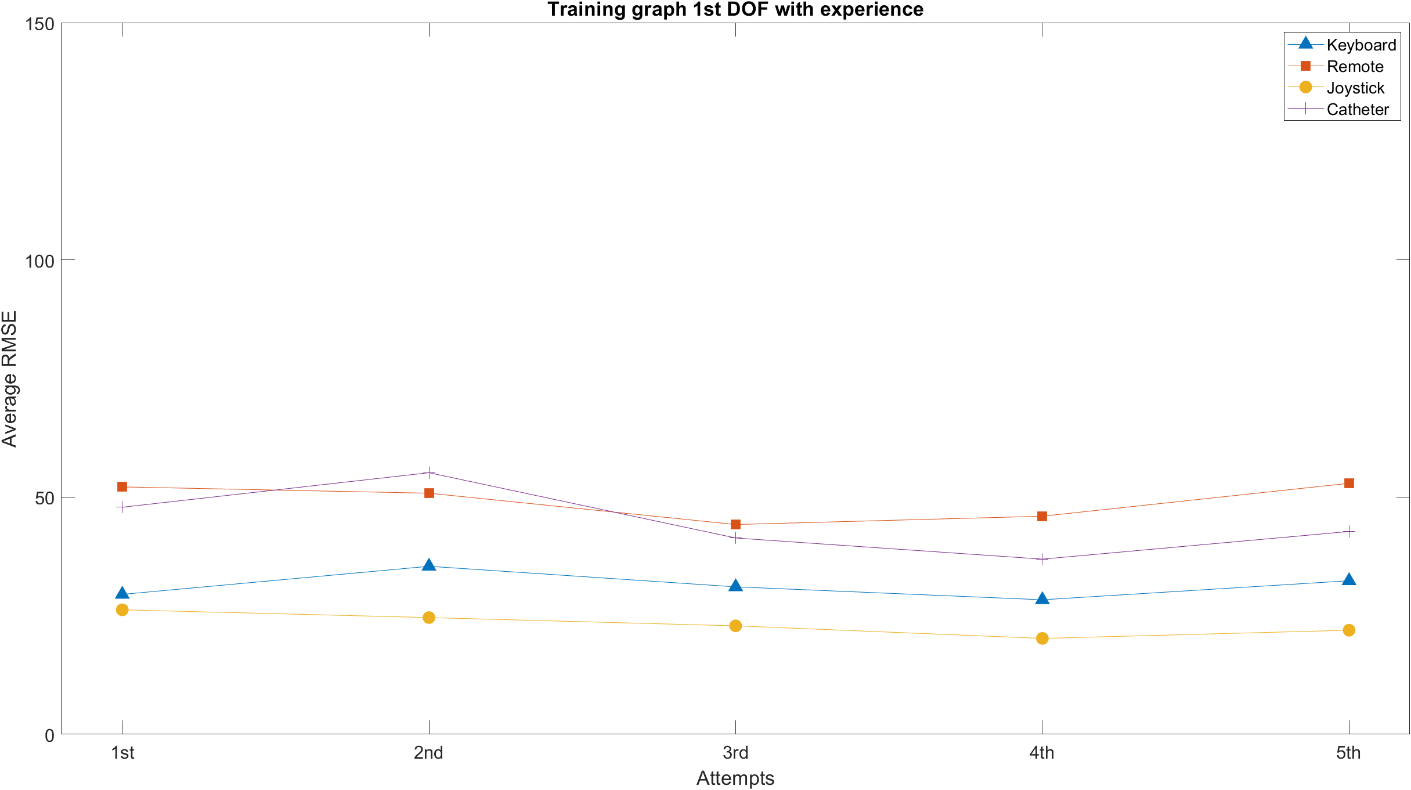
\includegraphics[width=1.0\textwidth]{img/1st/1stTrainExp.png}
   \caption{1st DOF RMSE per attempt, participant with experience}
   \label{img:1stTrainExp}
\end{figure}

\begin{figure}[ht]
   \centering
   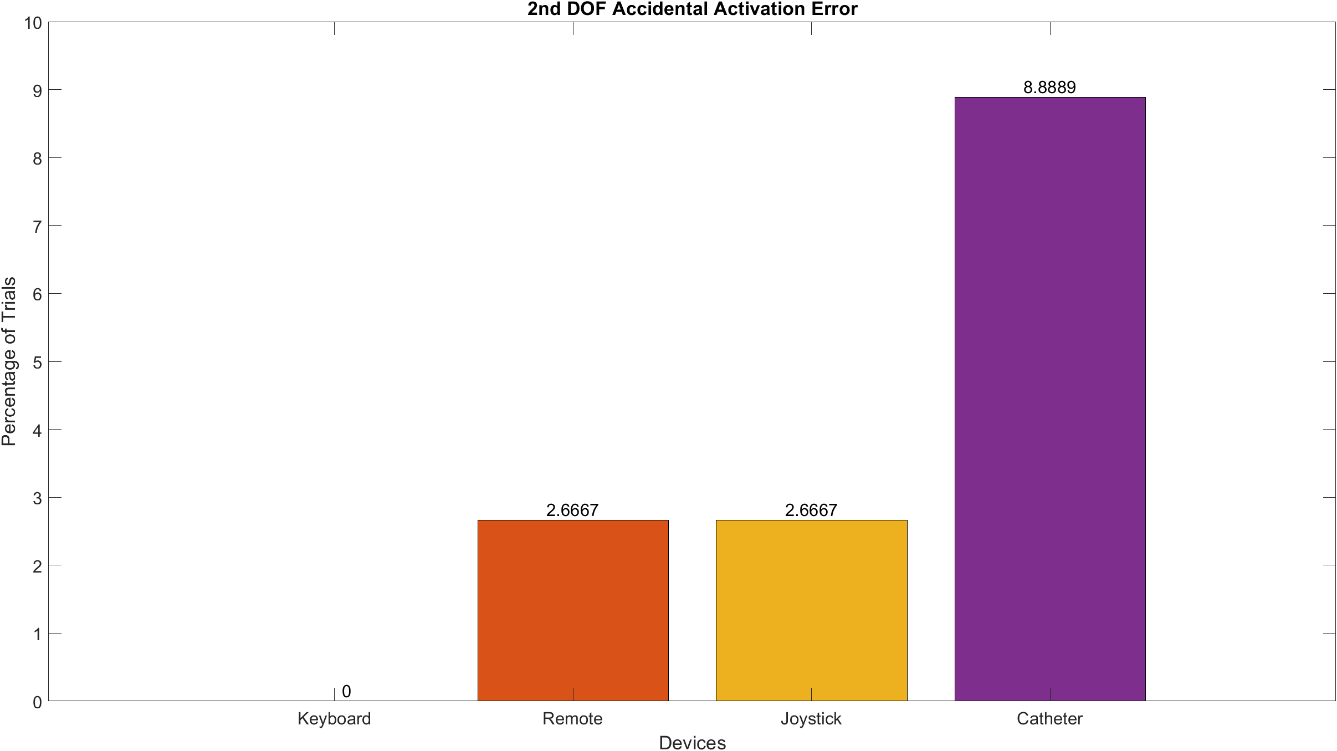
\includegraphics[width=1.0\textwidth]{img/1st/1stAct.png}
   \caption{2nd DOF Activation error while performing 1st DOF experiment}
   \label{img:1stAct}
\end{figure}

\begin{figure}[ht]
   \centering
   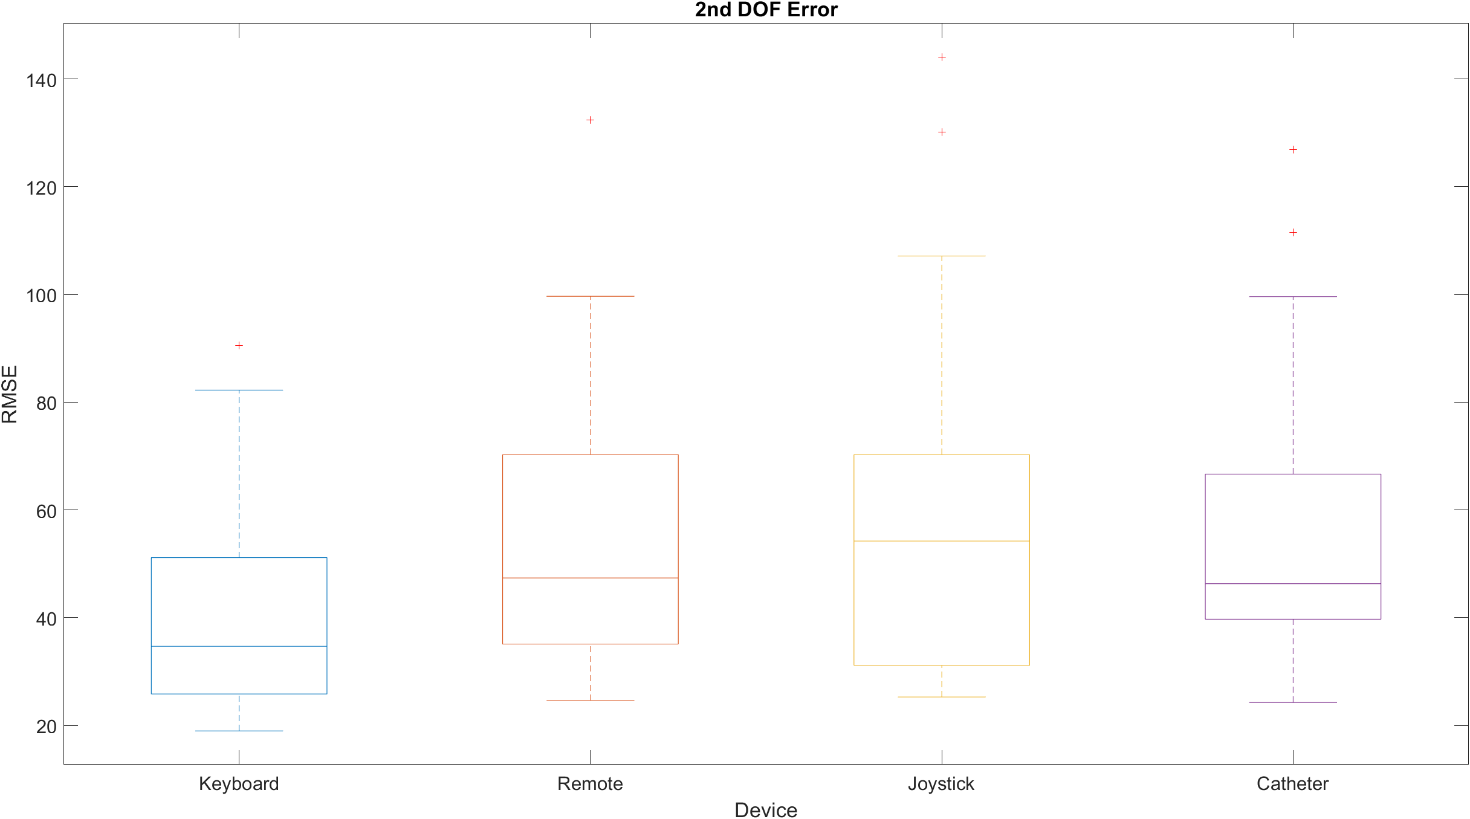
\includegraphics[width=1.0\textwidth]{img/2nd/2ndError.png}
   \caption{2nd DOF RMSE per device across all worlds}
   \label{img:2ndError}
\end{figure}

\begin{figure}[ht]
   \centering
   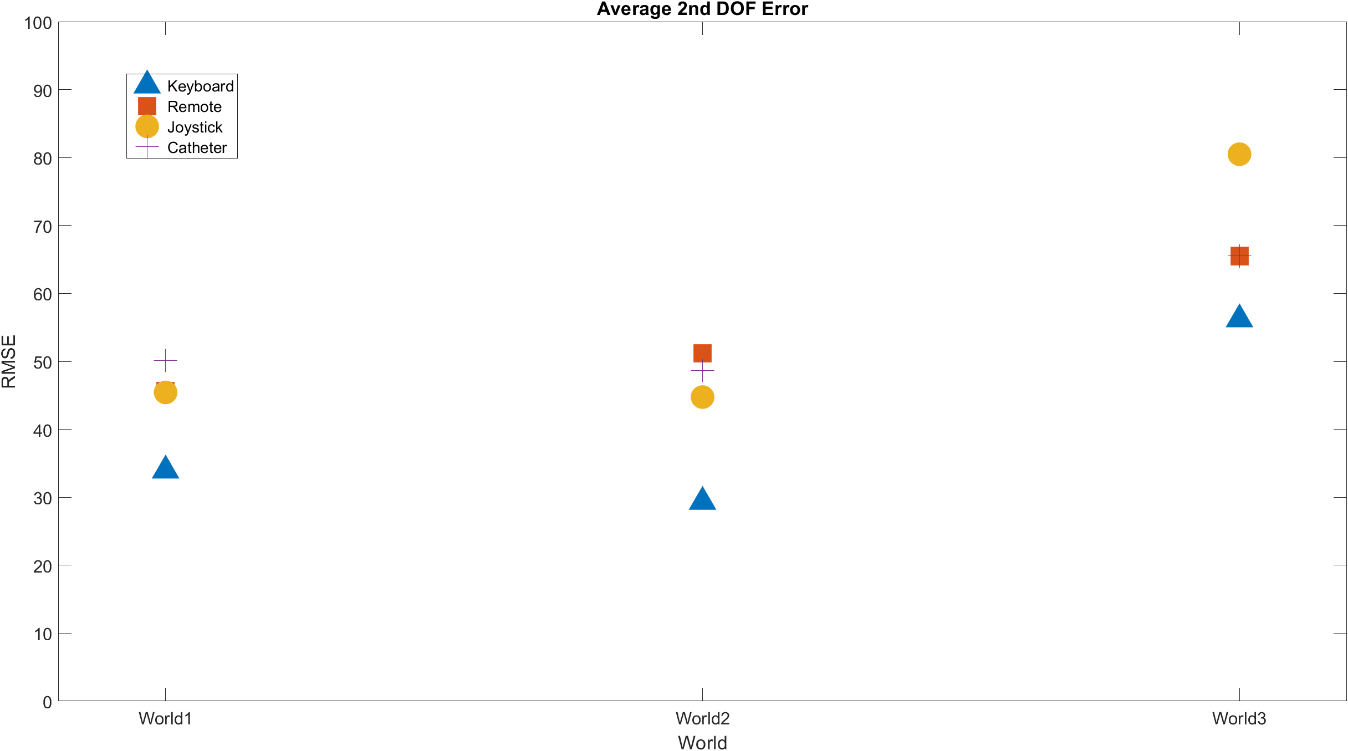
\includegraphics[width=1.0\textwidth]{img/2nd/2ndAvgError.png}
   \caption{2nd DOF RMSE per device at each world}
   \label{img:2ndAvgError}
\end{figure}

\begin{figure}[ht]
   \centering
   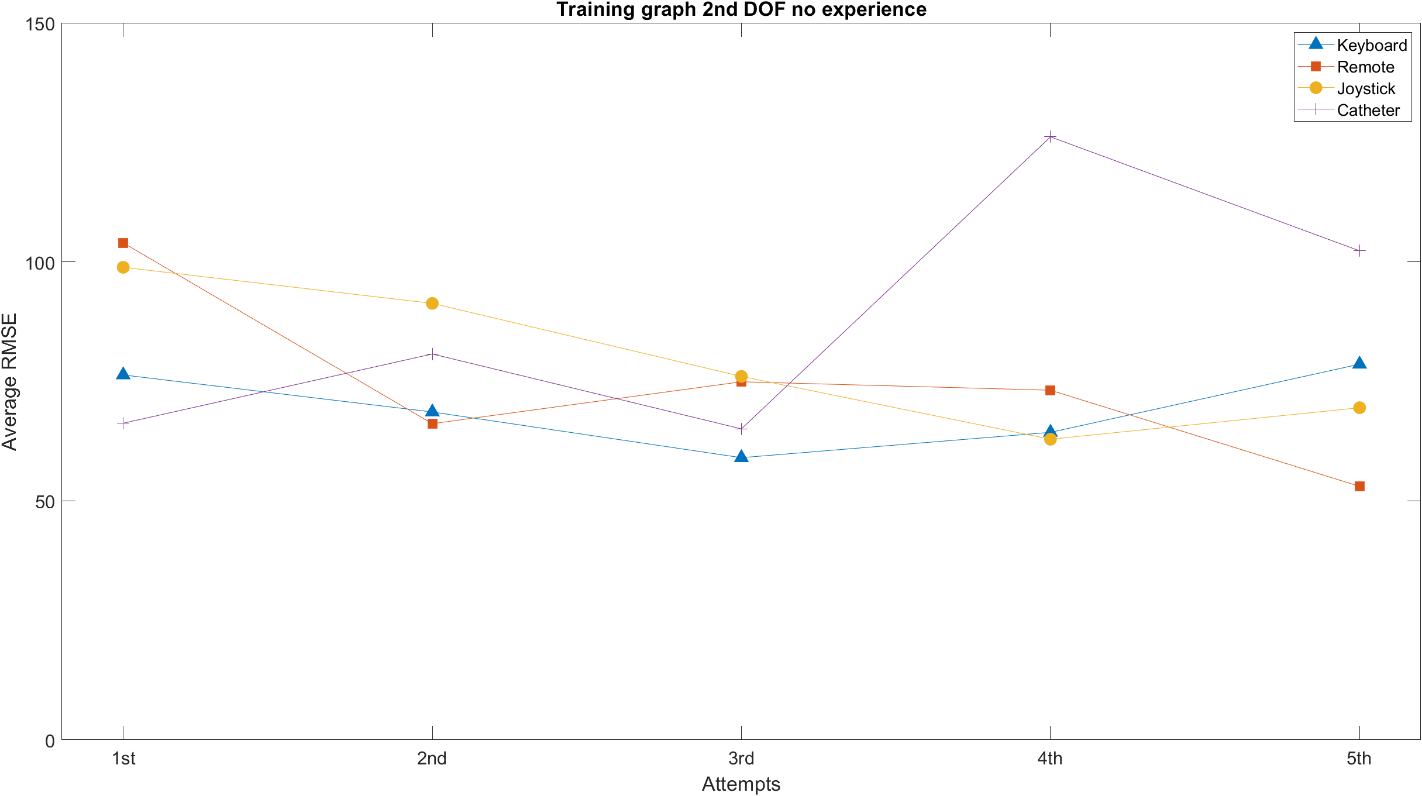
\includegraphics[width=1.0\textwidth]{img/2nd/2ndTrainNoExp.png}
   \caption{2nd DOF RMSE per attempt, participant with no experience}
   \label{img:2ndTrainNoExp}
\end{figure}

\begin{figure}[ht]
   \centering
   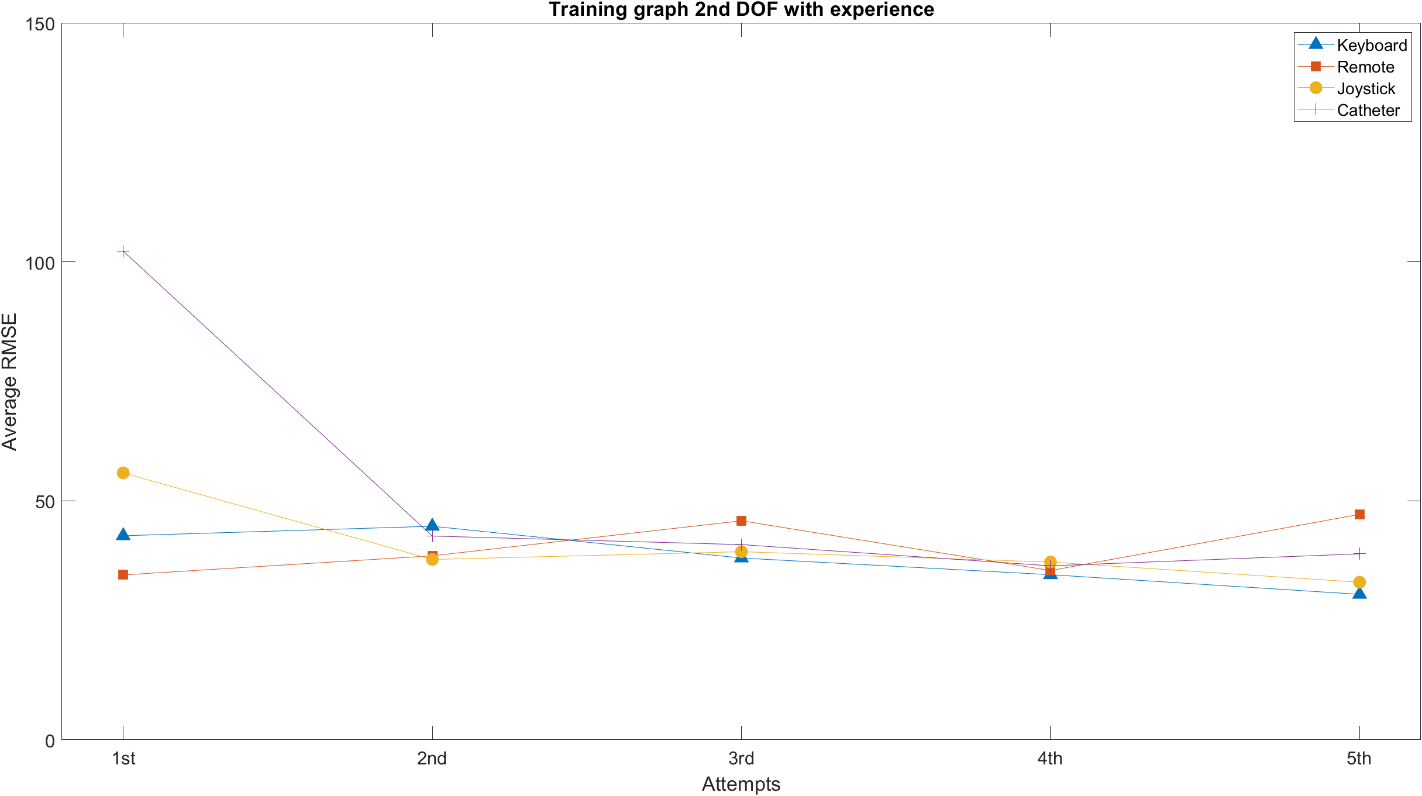
\includegraphics[width=1.0\textwidth]{img/2nd/2ndTrainExp.png}
   \caption{2nd DOF RMSE per attempt, participant with experience}
   \label{img:2ndTrainExp}
\end{figure}

\begin{figure}[ht]
   \centering
   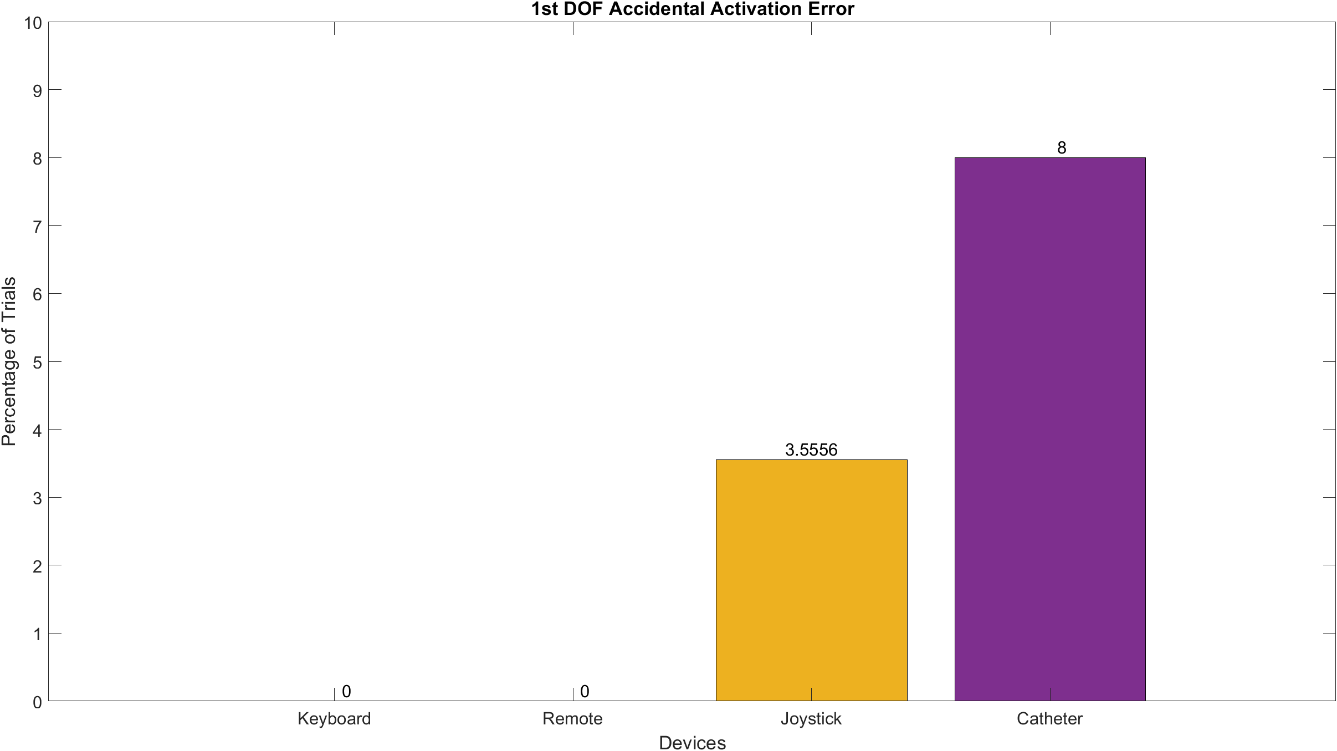
\includegraphics[width=1.0\textwidth]{img/2nd/2ndAct.png}
   \caption{1st DOF Activation error while performing 2nd DOF experiment}
   \label{img:2ndAct}
\end{figure}
\clearpage

\section{Experiment Maze}\label{sec:expmaze}
\subsection{Overview}\label{subsec:2ndover}
This experiment was designed to test the joint performance of the two DOF of every device. The objective is to navigate the tip of the simulated catheter (green square) through a one-way maze as shown in figure~\ref{img:maze}, until reaching the top part of the maze. The users were instructed (as shown in appendix~\ref{sec:apinst}) to navigate the maze keeping the maximum distance to the walls as possible, avoid collisions and reach the top wall of the maze in the minor time possible.\\

The simulation starts recording the data when the first movement of the user is detected. In case of colliding with a wall, the tip of the catheter stops moving and changes color from green to red (as shown in figure~\ref{img:mazeColl}), indicating a collisions status. In order clear the collision the user has to back off, any other movement that would keep the collision is not permitted and would not move the simulated catheter at all. Once the tip of the simulated catheter touches the upper wall (as shown in figure~\ref{img:mazeEnd}) the simulation stops.\\

In order to exploit all the capabilities of each device, two different mazes (worlds) were used for this experiment. The first maze (world1) has longer stretches in the 1st DOF, occasionally stopped by a short rotation movement, in order to simulate the first fast strokes the surgeons have to perform in order to reach the aortic arch, if a blockage is found, a small rotation is made and try to keep going forward. The second one (world2) with higher alternation between left/right and up/down movements, simulating scenarios where surgeons have to maneuver both DOF at the same time, example of that is when they cross the aortic valve~\cite{raptech}~\cite{anatomic}.\\

For this experiment three main metrics were measured, Time to complete the experiment, Number of collisions and Dimensionless squared Jerk. These metrics were selected since they enclose relevant information on the capabilities of the devices and how suitable to perform the tasks they are. Time to complete the tasks is of high importance, since one of the objectives of a Teleoperated robots is to reduce the radiation exposure both, to patients and practitioners. Number of collisions is important to give an insight of the maneuverability of every device (acceleration rate, deceleration rate, precision, among others) which is highly important for the patient safety. The dimensionless squared jerk has been previously used in similar studies to asses performance of catheter trajectories~\cite{dsj}~\cite{dsj2}, it is useful to describe the smoothness of the path as well as the accelerations and decelerations, while being independent of time and longitude of the path. The formula to calculate is described in equation~\ref{eq:dsjeq} where TP is the experiment time (from ti to te) and PL the path length of the trajectory followed by the user.\\

\begin{equation}
   \scalebox{1.5}{$Jd=(\int_{ti}^{te}(\dddot{x}(t))^2 + (\dddot{y}(t))^2 dt)*\frac{Tp^5}{PL^2}$}
   \centering
   \label{eq:dsjeq}
\end{equation}

For each one of the mazes every participant had to complete 5 repetitions, which means 10 randomly order repetitions per device. The repetitions were executed all, one device at a time; however, the devices were ordered randomly at the beginning of the experiment.\\

\begin{figure}[ht]
   \centering
   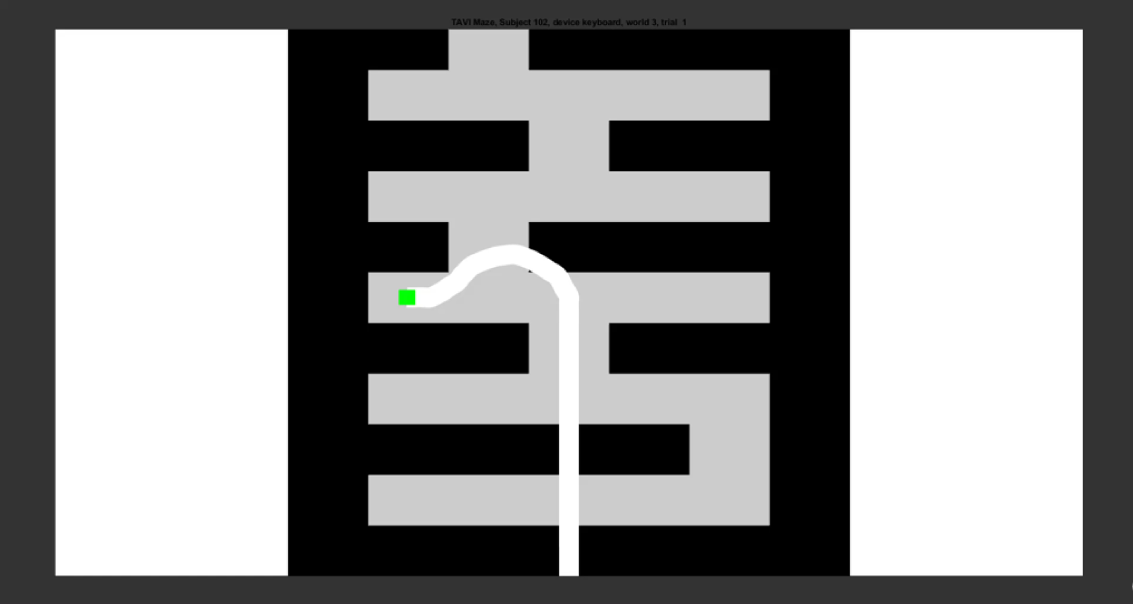
\includegraphics[width=1.0\textwidth]{img/maze/maze.png}
   \caption{Initial state of the experiment maze}
   \label{img:maze}
\end{figure}

\begin{figure}[ht]
   \centering
   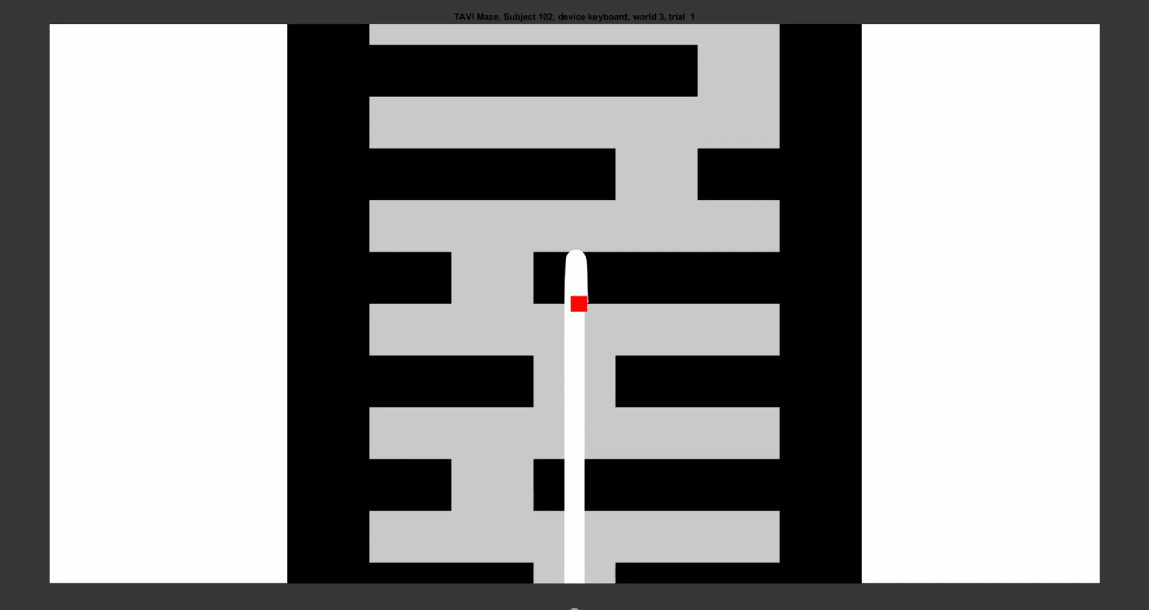
\includegraphics[width=1.0\textwidth]{img/maze/mazeColl.png}
   \caption{Collision during maze experiment}
   \label{img:mazeColl}
\end{figure}

\begin{figure}[ht]
   \centering
   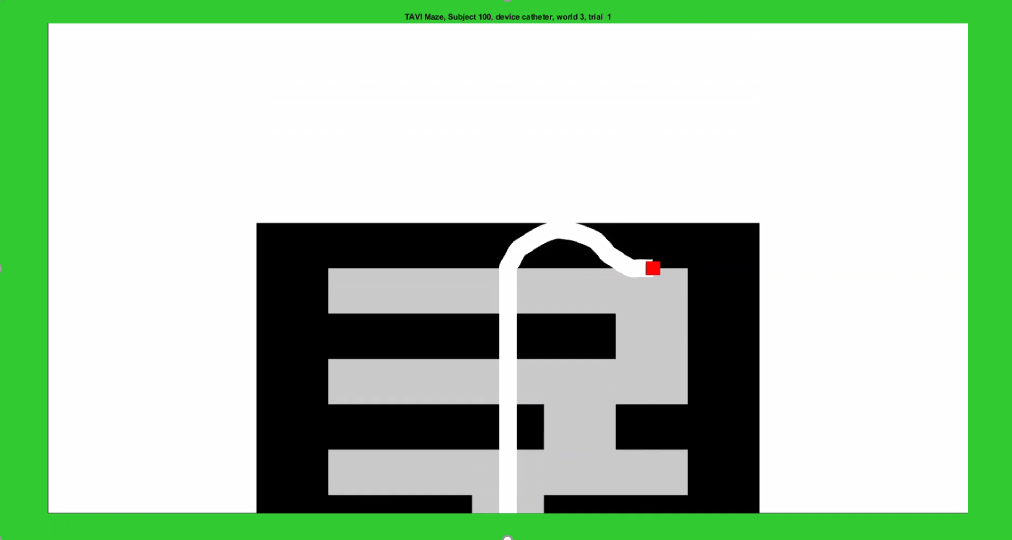
\includegraphics[width=1.0\textwidth]{img/maze/mazeEnd.png}
   \caption{End of maze experiment when colliding with upper wall}
   \label{img:mazeEnd}
\end{figure}

\subsection{Results}\label{subsec:2ndres}
The Time result of the experiment were not statistically conclusive, since interaction with P-Value $<$ 0.05 was always present in the comparison between all the devices. As can be seen in figure~\ref{img:mazeAvgTime}, the Keyboard and the Joystick had a close average time in world1, however, in world2 (with the long stretches) Keyboard dominates. This can be related to the easy control of the keyboard without any training given the immediate stop advantage, as mentioned in figure~\ref{img:adtable}, this allows the user to advance confident with high velocity without expecting a collision. Overall it can be observed in figure~\ref{img:mazeTime} that the lowest times were achieved with the Keyboard and Joystick, however, the distribution in the upper quartile in the joystick device as with the remote is widely spread, which as in the experiment for the 1st DOF and 2nd DOF may be attributed to the learning curve.\\

\begin{figure}[ht]
   \centering
   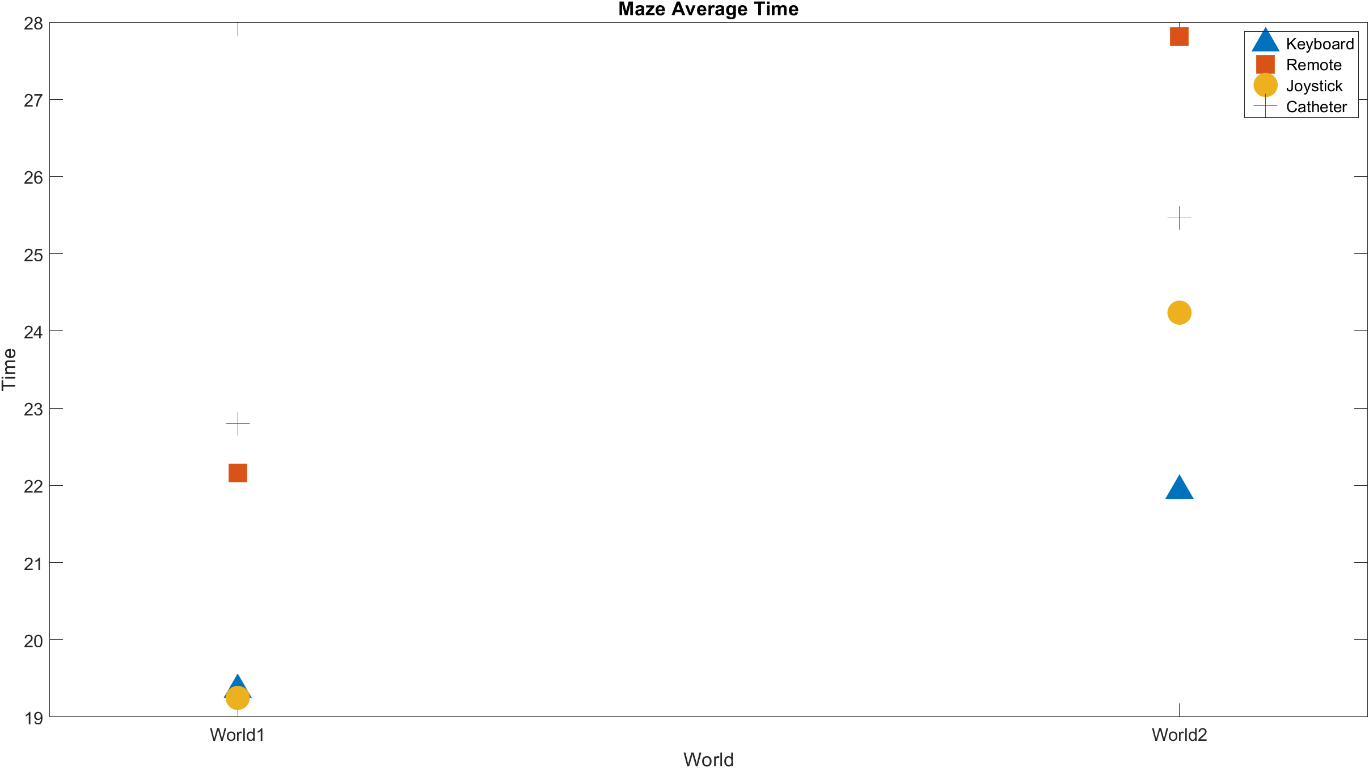
\includegraphics[width=1.0\textwidth]{img/maze/mazeAvgTime.png}
   \caption{Maze experiment average time per world}
   \label{img:mazeAvgTime}
\end{figure}

\begin{figure}[ht]
   \centering
   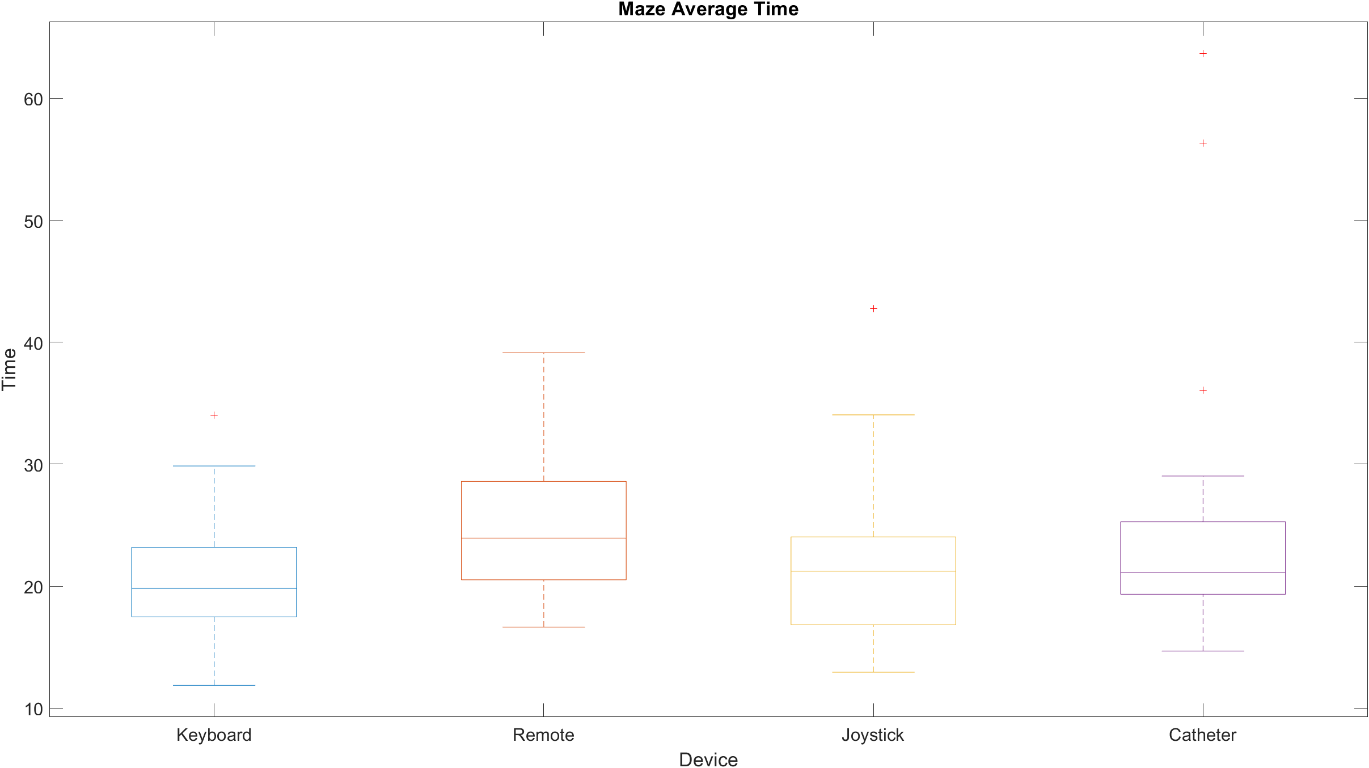
\includegraphics[width=1.0\textwidth]{img/maze/mazeTime.png}
   \caption{Maze experiment average time per device across all worlds}
   \label{img:mazeTime}
\end{figure}

\begin{figure}[ht]
   \centering
   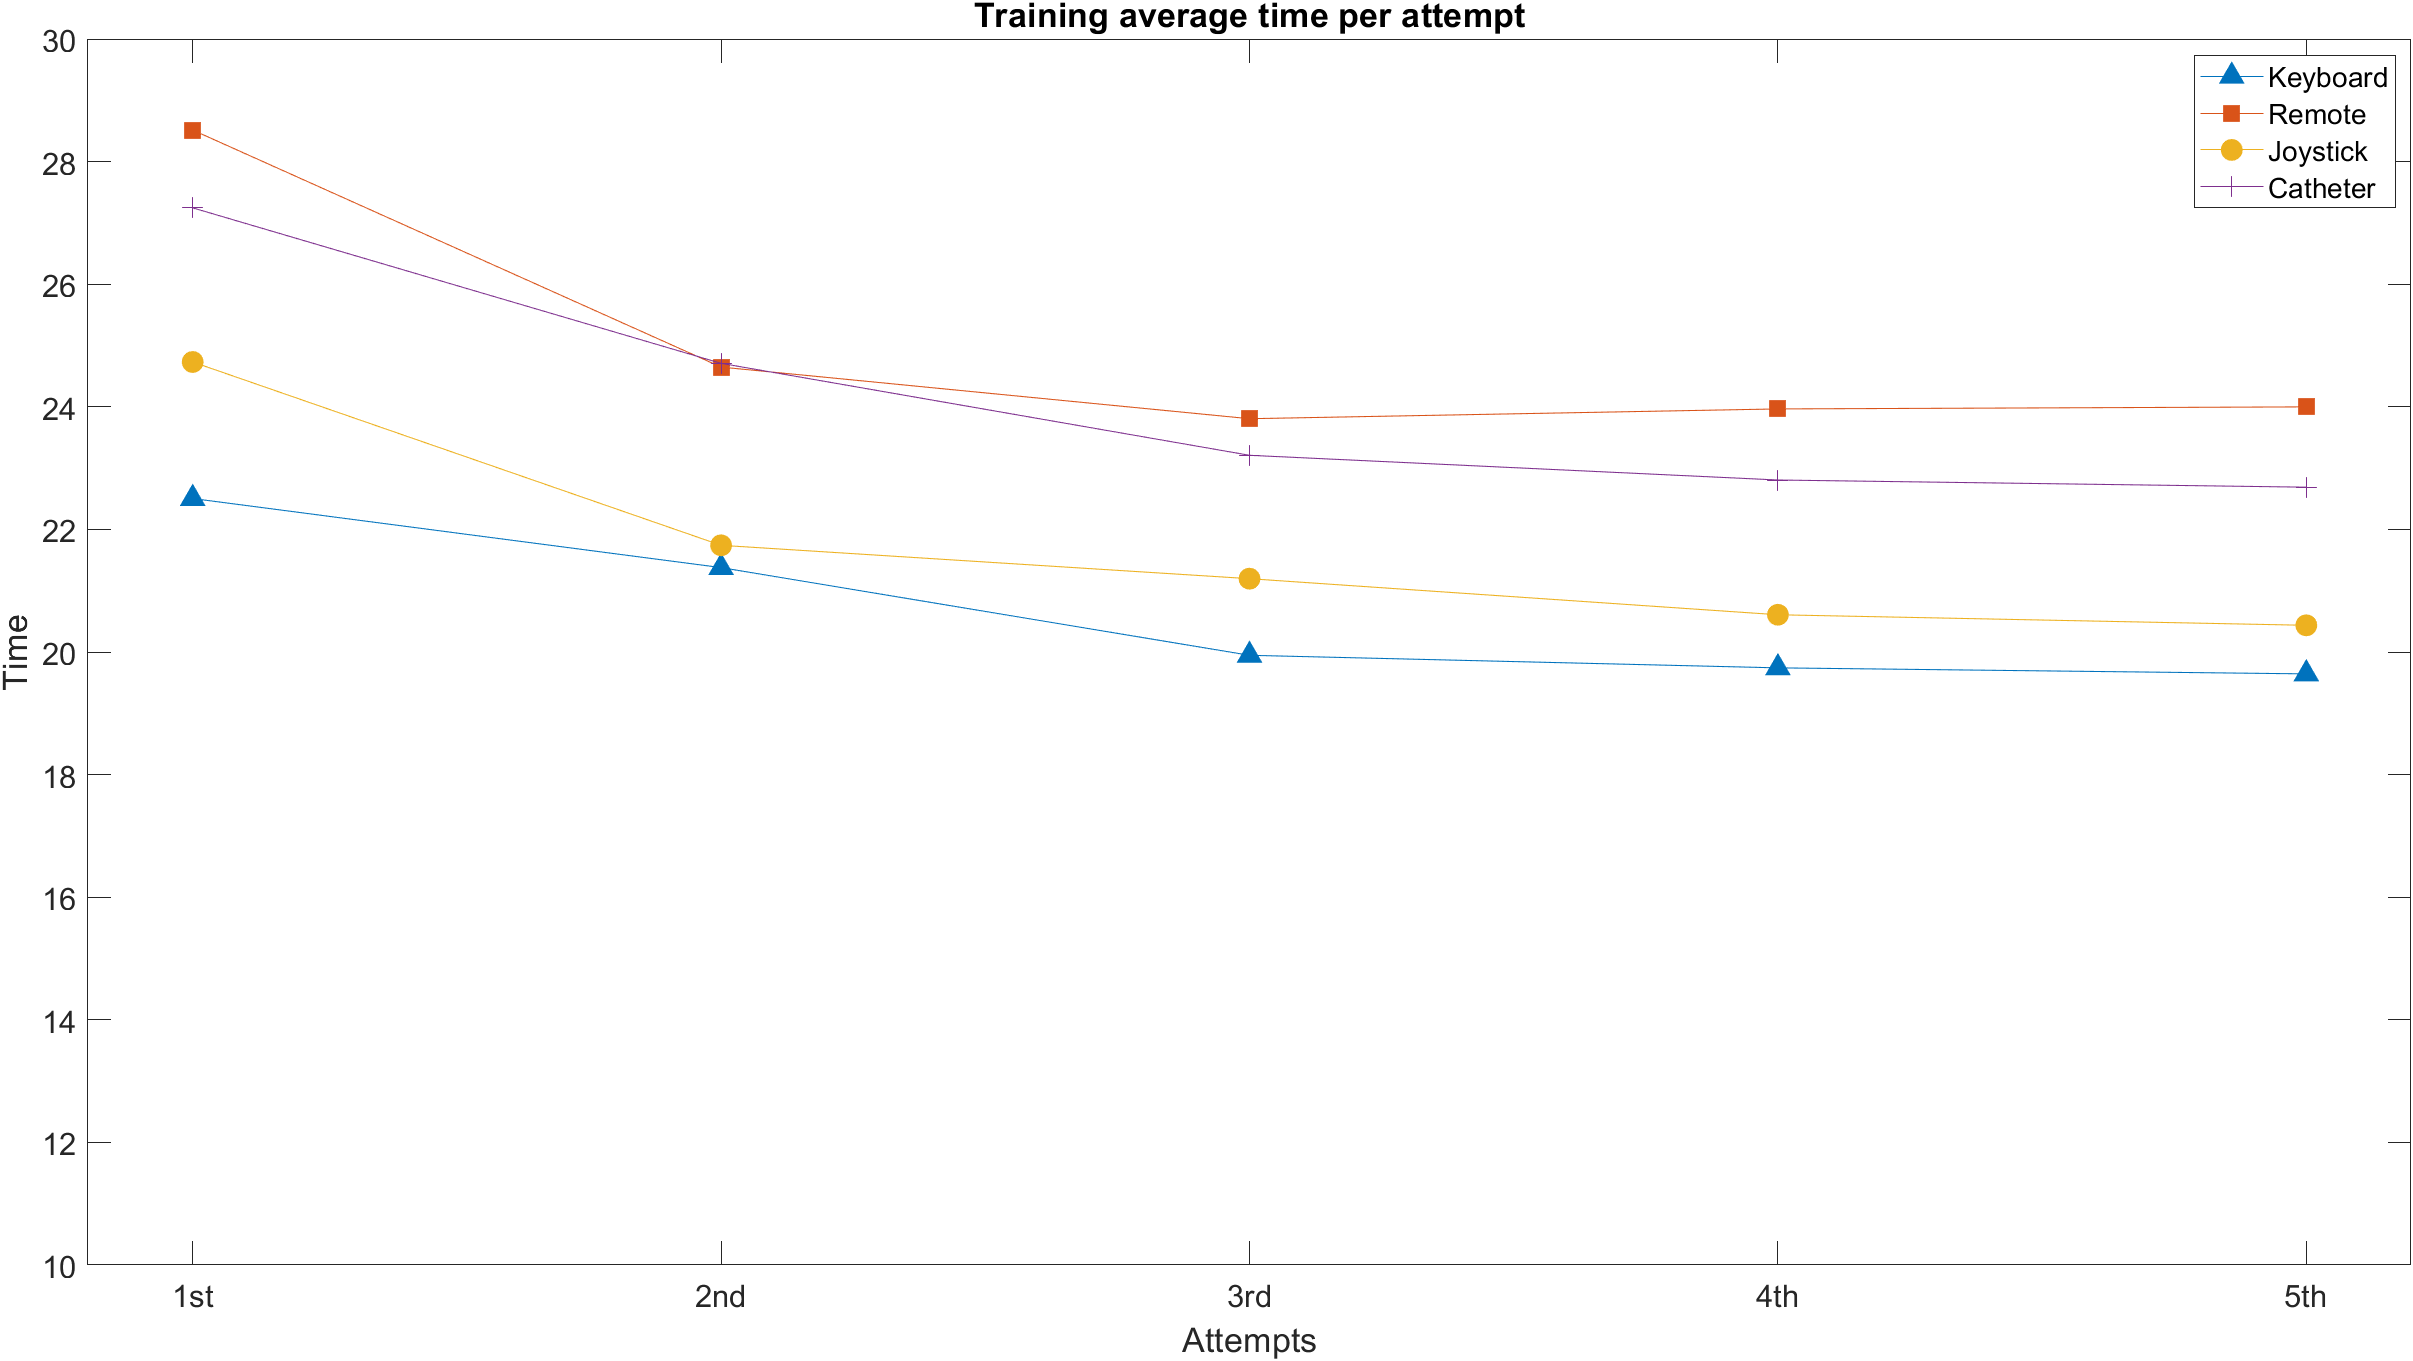
\includegraphics[width=1.0\textwidth]{img/maze/mazeTrainTime.png}
   \caption{Maze experiment time training curve of all participants}
   \label{img:mazeTrainTime}
\end{figure}

The average number of collisions (per repetition) shown in figure~\ref{img:mazeAvgColl} states that the Keyboard and Remote are significantly better than the Joystick and Catheter with a P-Value $<$ 0.01. This result gives again intuition about the importance of the advantages and disadvantages shown in figure~\ref{img:adtable}, if taking into account the information from figure~\ref{img:mazeAvgColl2}, where analogical sensor devices have a significant higher amount of collisions in world2 (world with longer stretches) than in world1, combined to the proneness of analogical sensor devices to overshot show how important is the participants training, and coming back to the Time results, it confirms how these collisions are related. This can be directly corroborated for the Joystick when putting together figure~\ref{img:mazeTrainColl} showing the collision training curve and figure~\ref{img:mazeTrainTime} showing the time training curve, where it can be appreciated how time per attempt go down as collisions per attempt go down.\\

\begin{figure}[ht]
   \centering
   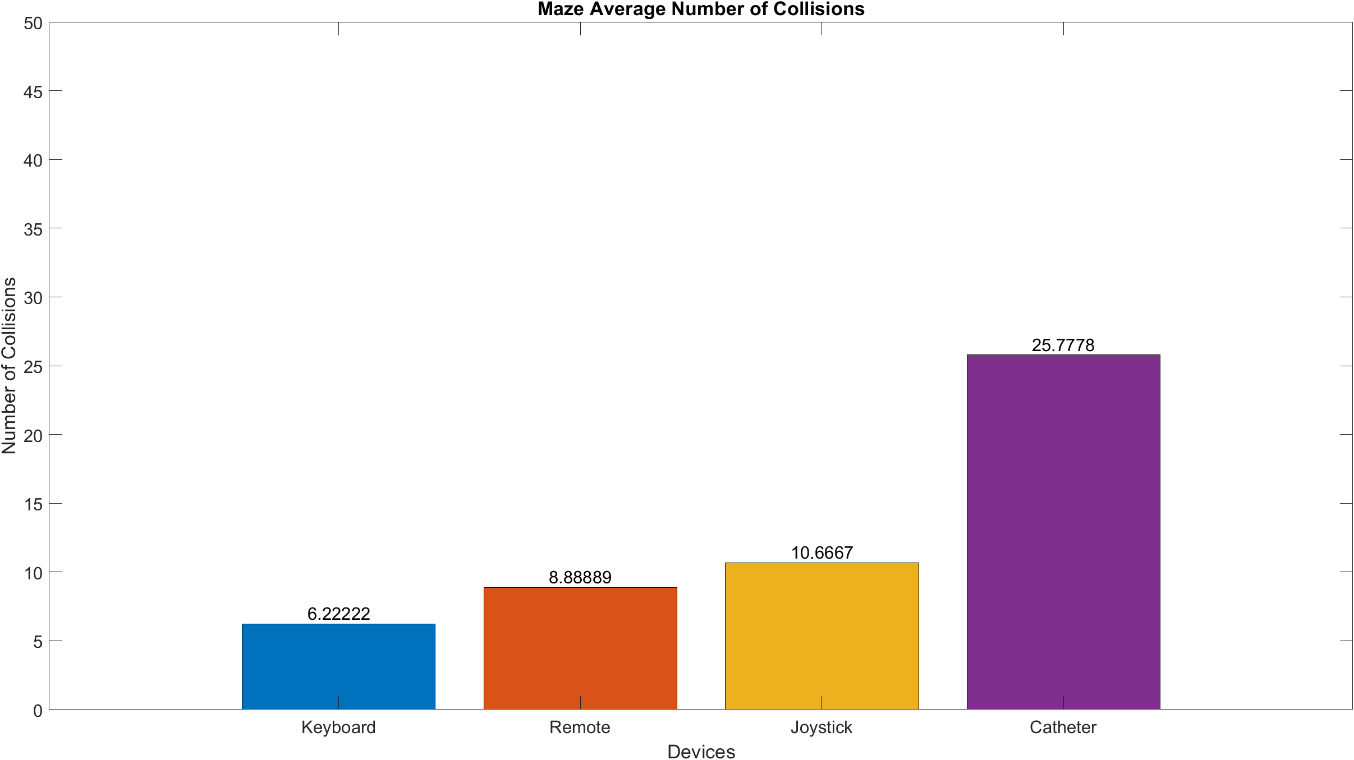
\includegraphics[width=1.0\textwidth]{img/maze/mazeAvgColl.png}
   \caption{Maze experiment average number of collisions per world}
   \label{img:mazeAvgColl}
\end{figure}

\begin{figure}[ht]
   \centering
   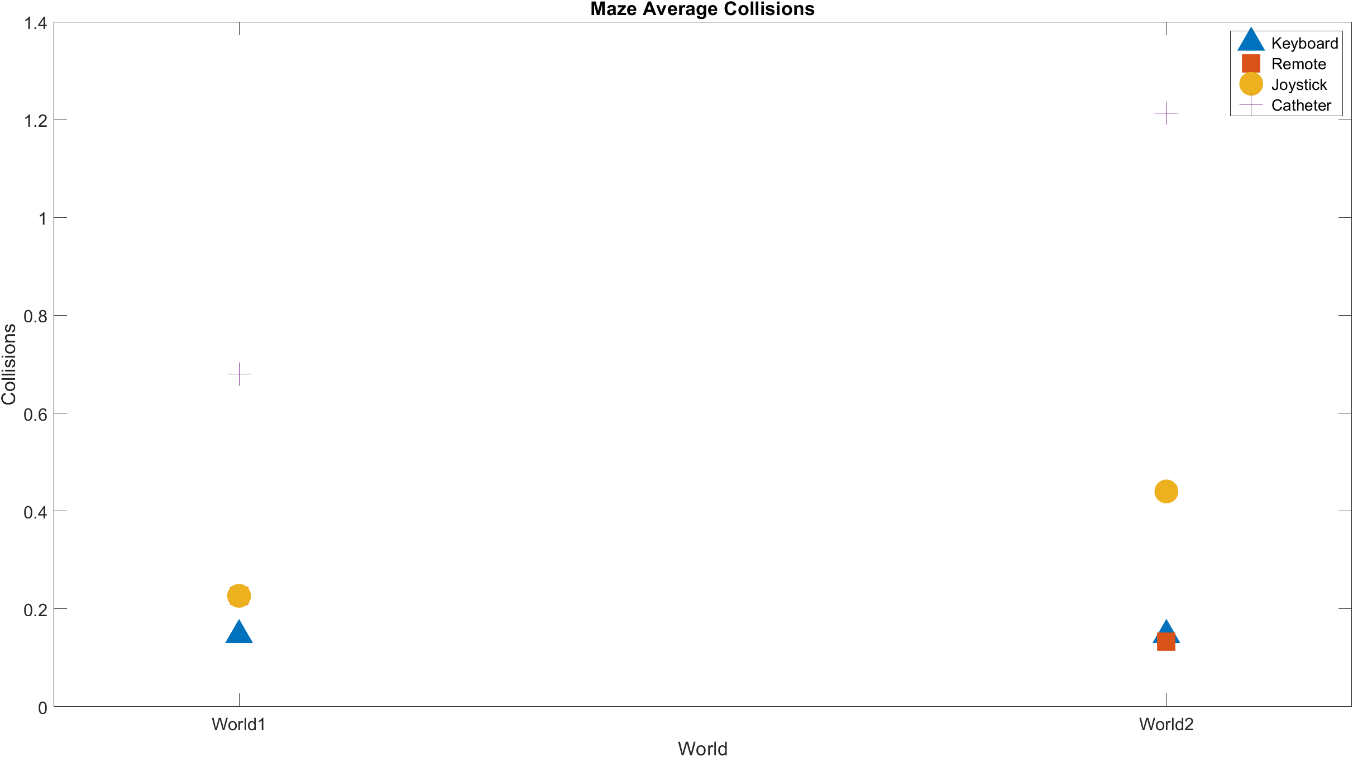
\includegraphics[width=1.0\textwidth]{img/maze/mazeAvgColl2.png}
   \caption{Maze experiment average number of collisions per device across all worlds}
   \label{img:mazeAvgColl2}
\end{figure}

\begin{figure}[ht]
   \centering
   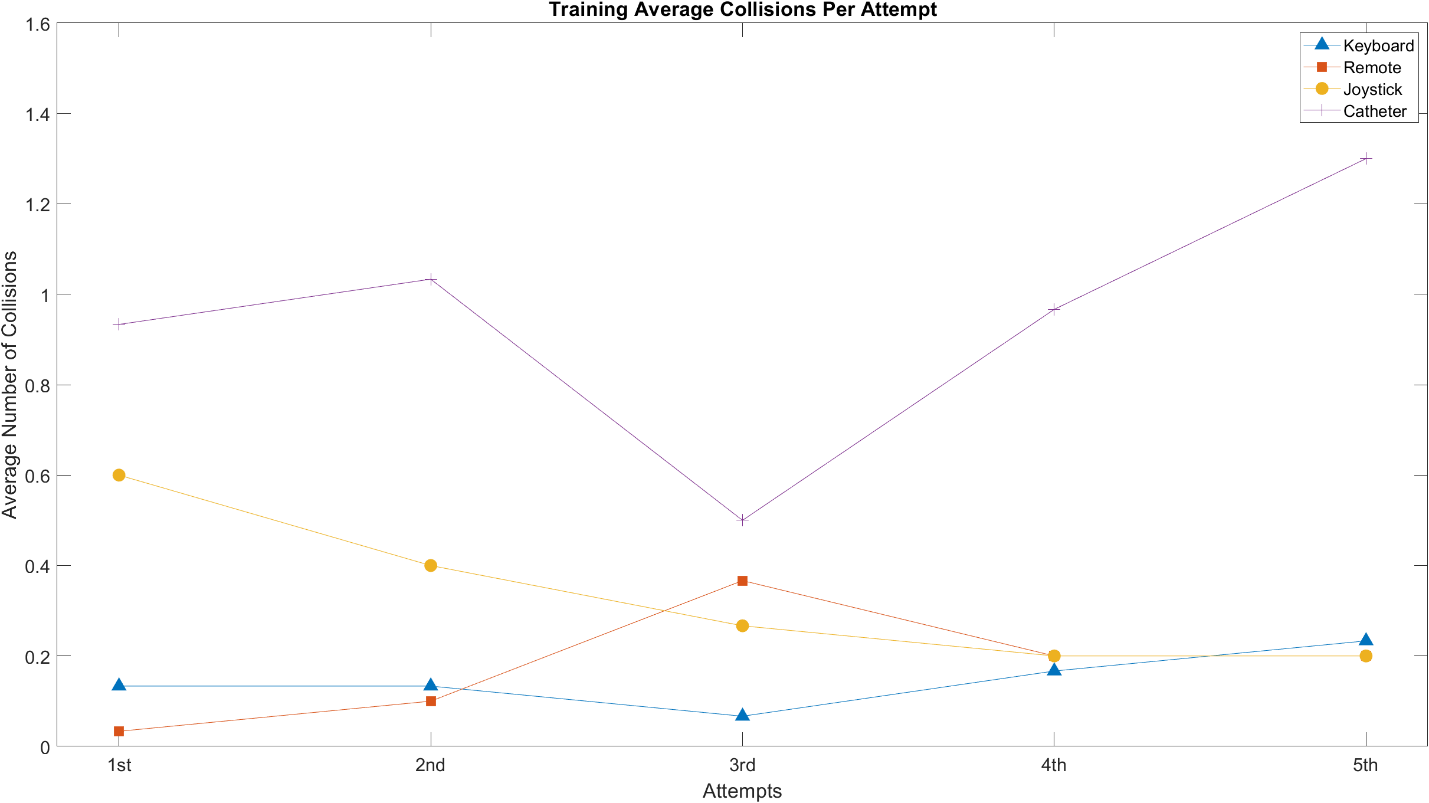
\includegraphics[width=1.0\textwidth]{img/maze/mazeTrainColl.png}
   \caption{Maze experiment number of collisions training curve of all participants}
   \label{img:mazeTrainColl}
\end{figure}

The joystick got a lower average Dimensionless Squared Jerk number in both worlds as shown in figure~\ref{img:mazeAvgDsj}, altough not significative due to interaction P-Value lower than 0.05, immedeatly followed by the keyboard device (figure~\ref{img:mazeDsj}). It is important to remark that part of the good result of the keyboard in the DSJ is due to the linear increment of thevelocity over time of the PressedTime-Velocity mapping, thus, if the function is changed to something non linear, this will have a high impact in this metric.\\

Also, it is important to remark how even though the Joystick had a worst performance than the keyboard in the collision average, and this collisions cause higher DSJ values, the performance overall in the DSJ was better. This may be caused due to the fact that the Keyboard can stop instactly, giving really high jerking values, which in a real world is also translated to high stress in the actuators.\\

\begin{figure}[ht]
   \centering
   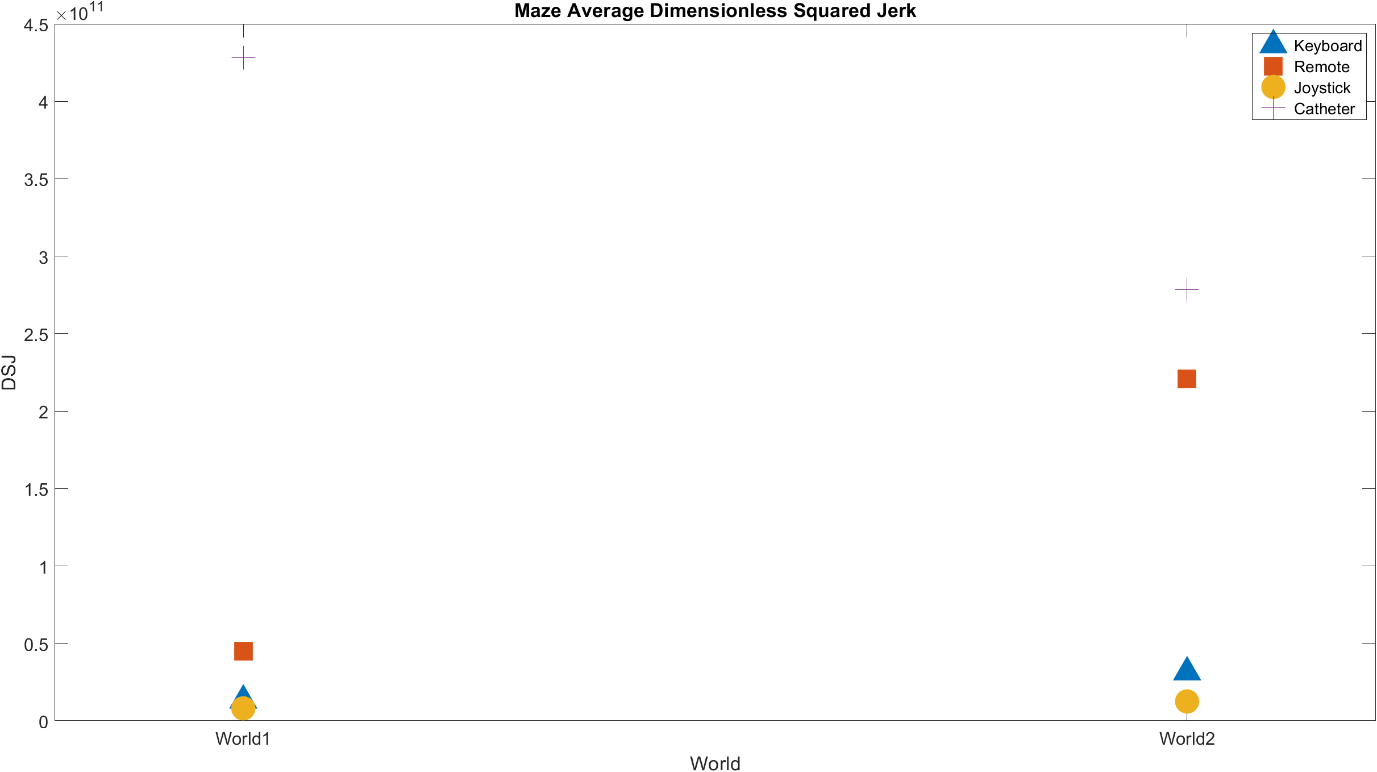
\includegraphics[width=1.0\textwidth]{img/maze/mazeAvgDsj.png}
   \caption{Maze experiment DSJ per world}
   \label{img:mazeAvgDsj}
\end{figure}

\begin{figure}[ht]
   \centering
   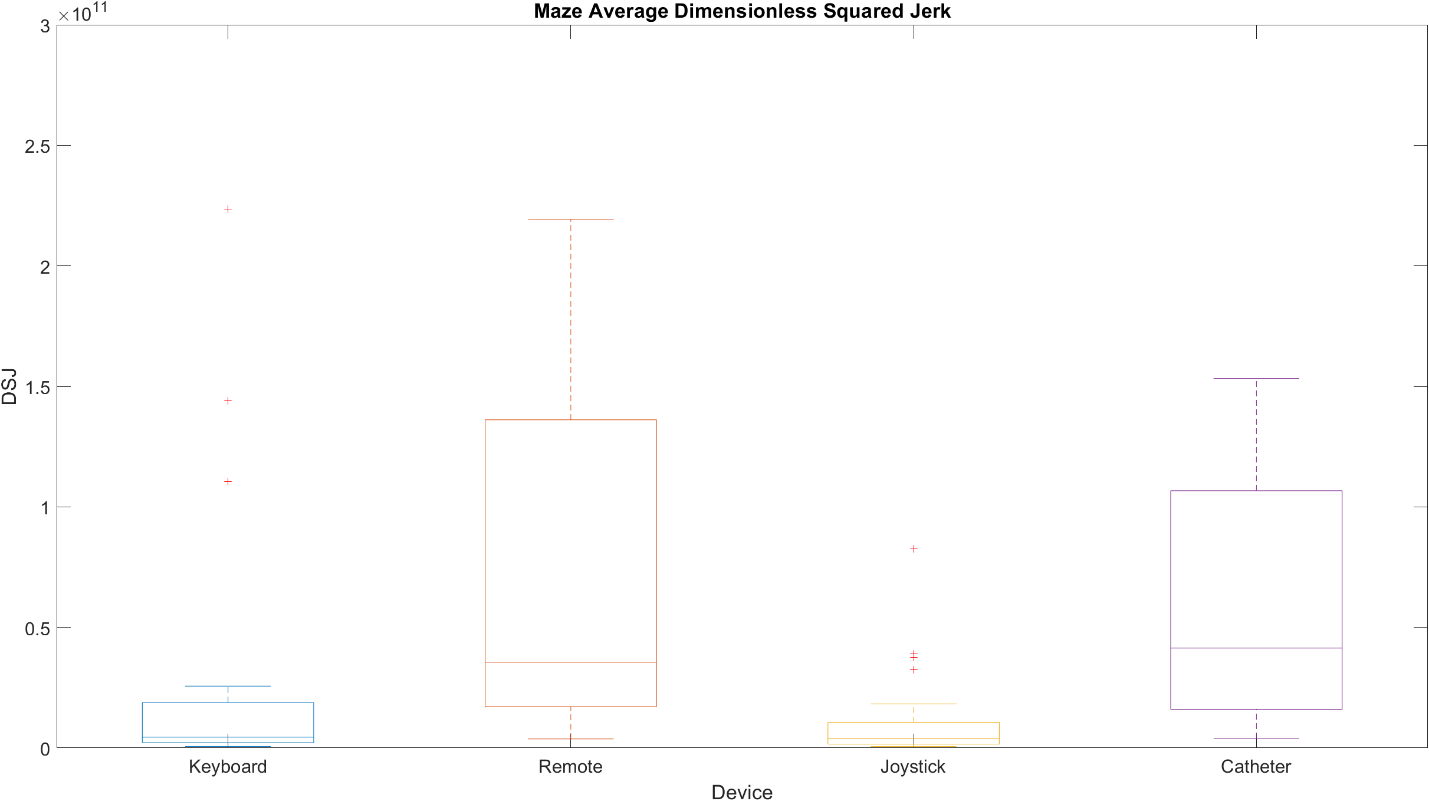
\includegraphics[width=1.0\textwidth]{img/maze/mazeDsj.png}
   \caption{Maze experiment DSJ per device across all worlds}
   \label{img:mazeDsj}
\end{figure}
\clearpage

\section{Poll Results}\label{sec:pollres}
After completing the experiment, each one of the participants was requested to answer questions about the performance of the devices and give any additional comment about the experiment/devices. The exact questions as they were handed to the participants can be found in appendix~\ref{sec:apsurv}.\\

Since the poll requested to enumerate the preference for the devices from 1-4, the figure~\ref{img:1stpoll}, figure~\ref{img:2ndpoll} and figure~\ref{img:overallpoll}, were calculated as a percentage by adding all the points each device got and dividing by the total amount of points. It can be seen for the 1st DOF device preference, the Joystick has the higher punctuation, followed by the keyboard and then the remote, leaving the catheter like last. Moreover, the 2nd DOF has in first place the Joystick again, in this case followed by the remote, then the keyboard and last the catheter device. The overall poll had the same results than the 1st DOF, but note that the difference between keyboard and remote got significantly reduced.\\

Another of the question asked to the participants was the experience with the devices, we can see in figure~\ref{img:expdev}, which shows how many participants out of the 15 declared experience in any of the devices, being the keyboard the most used, followed by the joystick.\\

The most relevant comments made by the participants are as follow:
\begin{itemize}
 \item  Remote appears to be significantly slower than keyboard in the 1st DOF
 \item Takes some time to operate the joystick, but with time it feels the easiest to use
 \item Rotation in joystick has too much dead zone and no low velocity
 \item 	(From Surgeon) The final user interface could use the Joystick as main device and the Remote as detachable device for being able to operate near the patient if necessary.\\
\end{itemize}

\begin{figure}[ht]
   \centering
   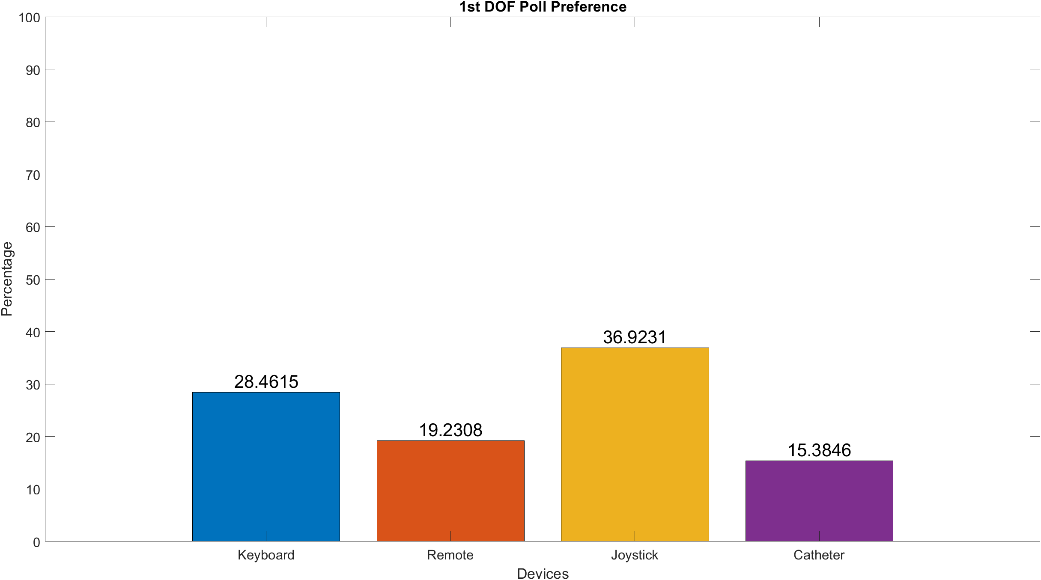
\includegraphics[width=1.0\textwidth]{img/poll/1stpoll.png}
   \caption{Participants percentage of preference per device on the 1st DOF}
   \label{img:1stpoll}
\end{figure}

\begin{figure}[ht]
   \centering
   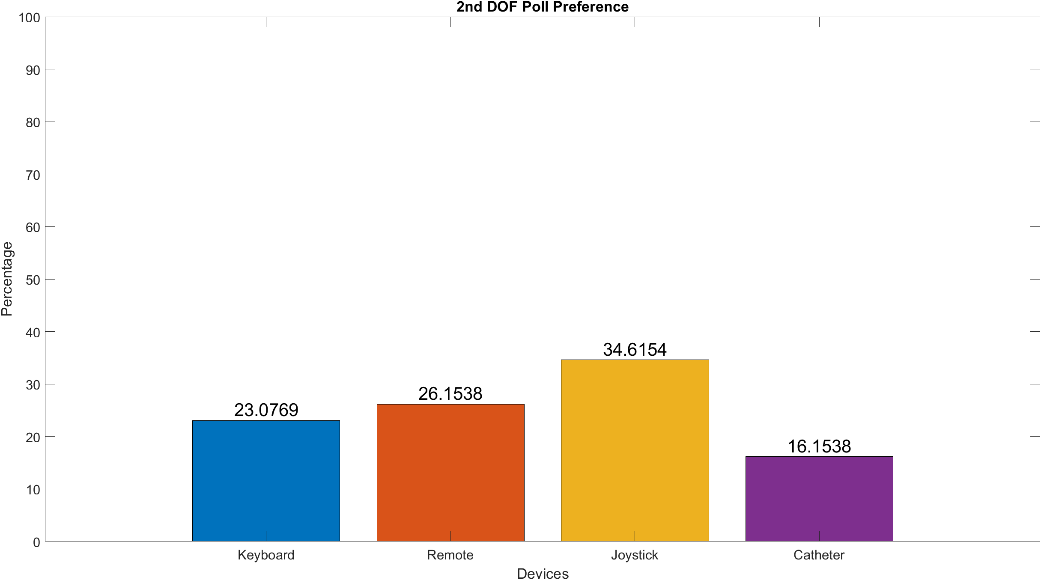
\includegraphics[width=1.0\textwidth]{img/poll/2ndpoll.png}
   \caption{Participants percentage of preference per device on the 2nd DOF}
   \label{img:2ndpoll}
\end{figure}

\begin{figure}[ht]
   \centering
   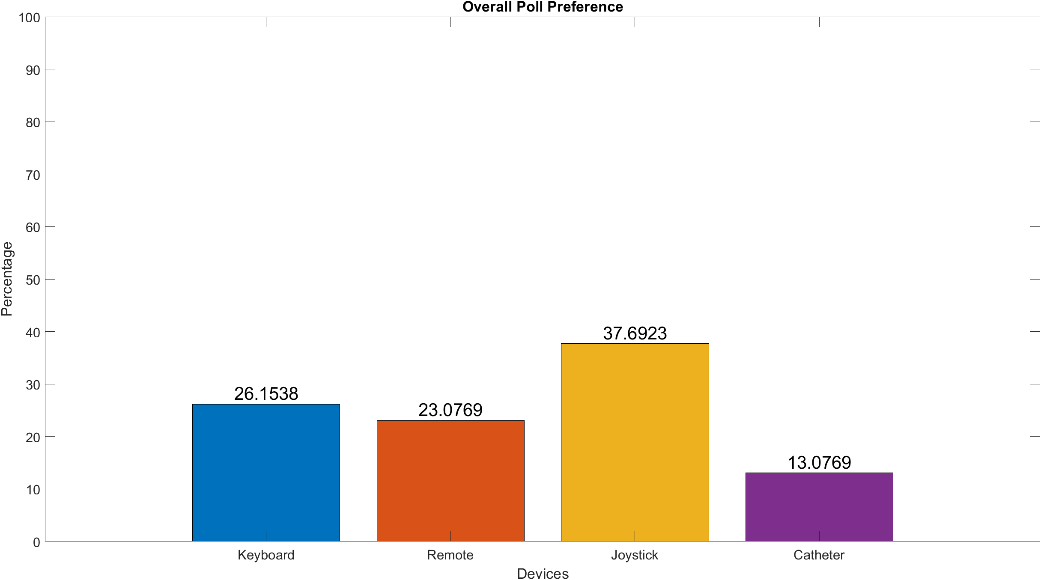
\includegraphics[width=1.0\textwidth]{img/poll/overallpoll.png}
   \caption{Participants percentage of preference per device on the overall}
   \label{img:overallpoll}
\end{figure}

\begin{figure}[ht]
   \centering
   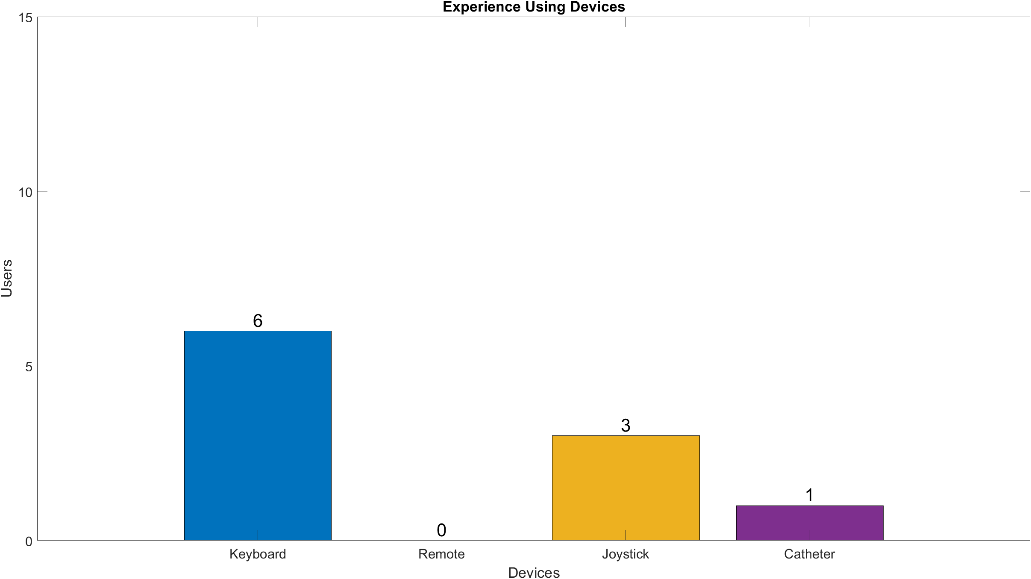
\includegraphics[width=1.0\textwidth]{img/poll/expdev.png}
   \caption{Number of participants with experience with each master device}
   \label{img:expdev}
\end{figure}


